\documentclass[compress]{beamer}
\usepackage{ifthen,verbatim}

\newcommand{\isnote}{}
\xdefinecolor{lightyellow}{rgb}{1.,1.,0.25}
\xdefinecolor{darkblue}{rgb}{0.1,0.1,0.7}

%% Uncomment this to get annotations
%% \def\notes{\addtocounter{page}{-1}
%%            \renewcommand{\isnote}{*}
%% 	   \beamertemplateshadingbackground{lightyellow}{white}
%%            \begin{frame}
%%            \frametitle{Notes for the previous page (page \insertpagenumber)}
%%            \itemize}
%% \def\endnotes{\enditemize
%% 	      \end{frame}
%%               \beamertemplateshadingbackground{white}{white}
%%               \renewcommand{\isnote}{}}

%% Uncomment this to not get annotations
\def\notes{\comment}
\def\endnotes{\endcomment}

\setbeamertemplate{navigation symbols}{}
\setbeamertemplate{headline}{\mbox{ } \hfill
\begin{minipage}{5.5 cm}
\vspace{-0.75 cm} \small
\end{minipage} \hfill
\begin{minipage}{4.5 cm}
\vspace{-0.75 cm} \small
\begin{flushright}
\ifthenelse{\equal{\insertpagenumber}{1}}{}{Jim Pivarski \hspace{0.2 cm} \insertpagenumber\isnote/\pageref{numpages}}
\end{flushright}
\end{minipage}\mbox{\hspace{0.2 cm}}\includegraphics[height=1 cm]{../cmslogo} \hspace{0.1 cm} \includegraphics[height=1 cm]{../tamulogo} \hspace{0.01 cm} \vspace{-1.05 cm}}

\begin{document}
\begin{frame}
\vfill
\begin{center}
\textcolor{darkblue}{\Large Summary of Current Knowledge of \\ \vspace{0.2 cm} Global Track-based Alignment}

\vfill
\begin{columns}
\column{0.3\linewidth}
\begin{center}
\large
\textcolor{darkblue}{Jim Pivarski}

\vspace{0.2 cm}
Alexei Safonov
\end{center}
\end{columns}

\begin{columns}
\column{0.3\linewidth}
\begin{center}
\scriptsize
{\it Texas A\&M University}
\end{center}
\end{columns}

\vfill
20 March, 2009

\end{center}
\end{frame}

%% \begin{notes}
%% \item This is the annotated version of my talk.
%% \item If you want the version that I am presenting, download the one
%% labeled ``slides'' on Indico (or just ignore these yellow pages).
%% \item The annotated version is provided for extra detail and a written
%% record of comments that I intend to make orally.
%% \item Yellow notes refer to the content on the {\it previous} page.
%% \item All other slides are identical for the two versions.
%% \end{notes}

\small

\begin{frame}
\frametitle{Understanding old plots}
\begin{itemize}\setlength{\itemsep}{0.2 cm}
\item A lot has been learned since the first CRAFT globalMuons
\item Now would be a good time to summarize the results, as they're
  currently understood
\begin{itemize}\setlength{\itemsep}{0.2 cm}
\item No rotation/twist with respect to the tracker
\item Magnetic field errors $\lesssim$ statistical with two-bin approach
\item Progress in understanding the ``sawtooth effect'' \textcolor{darkblue}{(new)}
\item ``Deterioration'' of globalMuons in cosmic \mbox{splitting resolved \textcolor{darkblue}{(new)}\hspace{-1 cm}}
\item Residuals distributions of hits that pull the fit
\item Incompleteness of the current alignment
\item Access to all 6 parameters with non-Gaussian fits \textcolor{darkblue}{(new)}
\item Alignment software updates \textcolor{darkblue}{(new)}
% \item Importance of single scattering
\item A comment about HIP and MillePede approaches
\end{itemize}
\end{itemize}
\end{frame}

\scriptsize

\begin{frame}
\frametitle{No significant rotation or twist}
\textcolor{darkblue}{Residuals merged across stations and sectors (Nov '08)} \hfill \textcolor{darkblue}{chamber alignments \mbox{(Feb '09)\hspace{-0.4 cm}}}

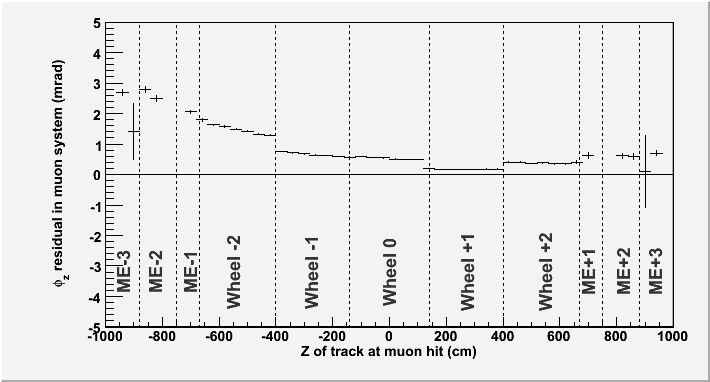
\includegraphics[height=3.7 cm]{phiresid_from_muon.png} \hfill 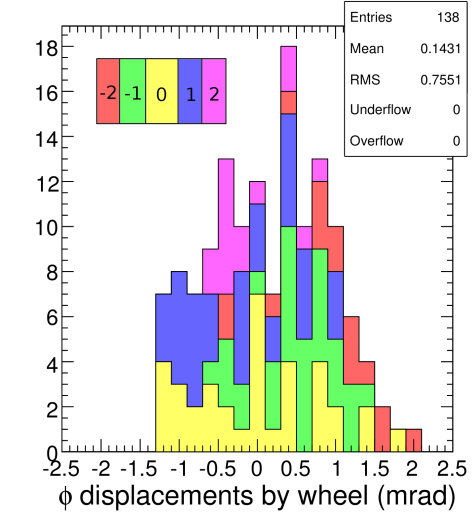
\includegraphics[height=3.7 cm]{report2_phibywheel.png}

\vfill
\begin{columns}
\column{0.4\linewidth}
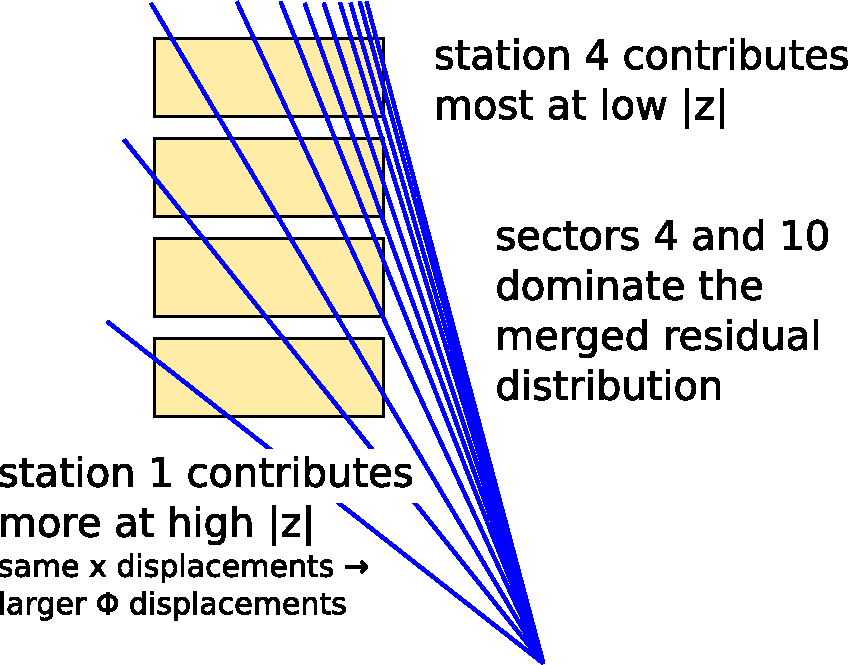
\includegraphics[width=\linewidth]{merged_residuals_mix_chambers.pdf}

\column{0.6\linewidth}
\begin{itemize}
\item Tracker alignment changed between Nov and Feb, but not enough to
  explain difference

\item Failing to separate residuals by chamber allows a few chambers
  to dominate wheel- by-wheel averages because of steep $\phi$,
  $\theta$ cosmic ray distributions

\item 16/50 chambers in wheel $-$2 have an average $\phi$ displacement of
  0.7~mrad, spread of 0.5

\item Chamber-by-chamber alignment is important!
\end{itemize}
\end{columns}
\end{frame}

\begin{frame}
\frametitle{$\vec{B}(\vec{x})$ is well controlled}

\vspace{-0.5 cm}
\begin{columns}
\column{0.5\linewidth}

\vspace{0.7 cm}
\begin{itemize}
\item Below: re-create \mbox{the ``alignment map''\hspace{-0.5 cm}} plots with new $\vec{B}(\vec{x})$ simulation
\begin{itemize}
\item \textcolor{red}{\scriptsize Red points show insensitivity of alignment to $\vec{B}(\vec{x})$}
\item \textcolor{blue}{\scriptsize Blue test correctness of \mbox{new $\vec{B}(\vec{x})$\hspace{-1 cm}}}
\item \scriptsize $\vec{B}(\vec{x})$ differs by up to 30\%
\end{itemize}
\item Bottom-right: how each alignment bin changes \mbox{(statistical errors are $\sim$0.5~mm)\hspace{-1 cm}}
\end{itemize}

\column{0.5\linewidth}
``Alignment map'' with $\vec{B}$ error tracer \mbox{in \textcolor{blue}{blue}\hspace{-1 cm}}

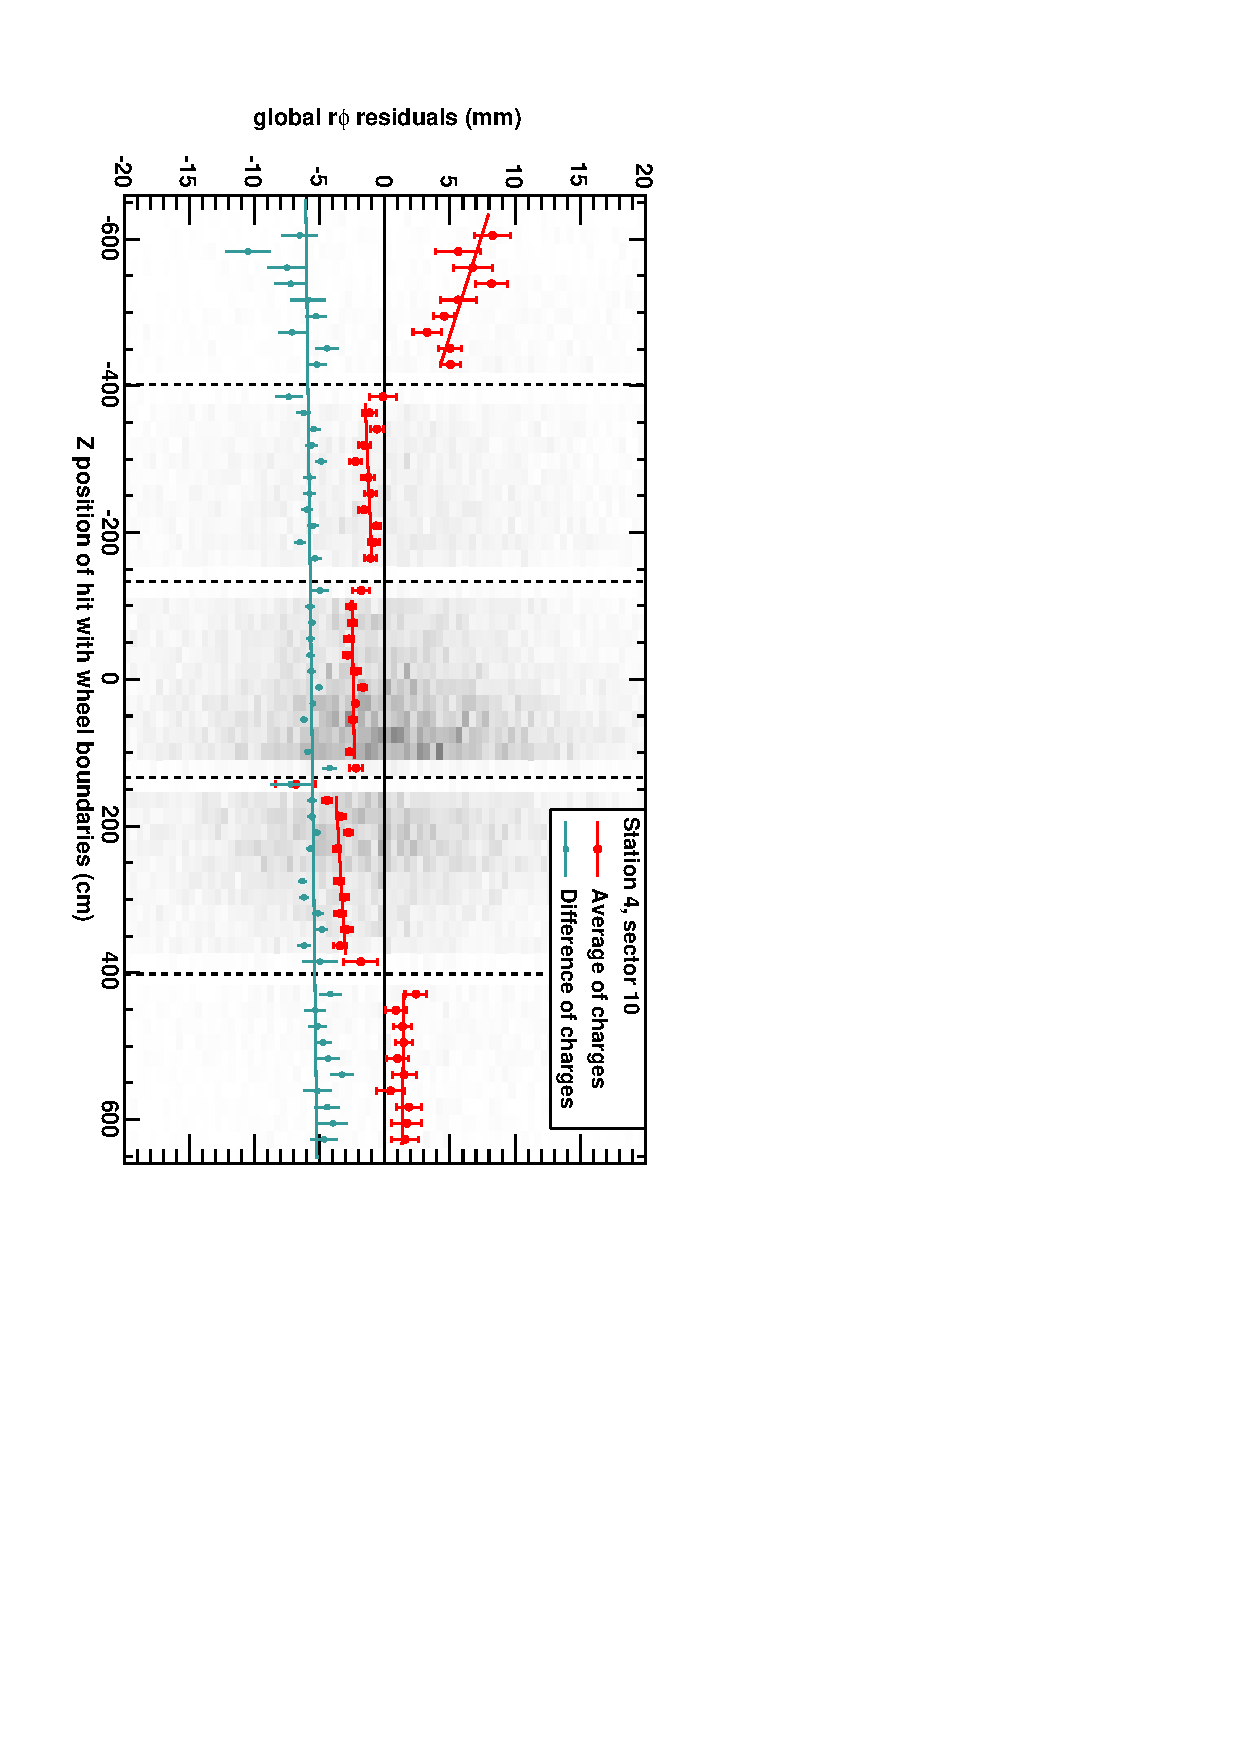
\includegraphics[height=\linewidth, angle=90]{demo_of_bfield.pdf}
\end{columns}

\vfill
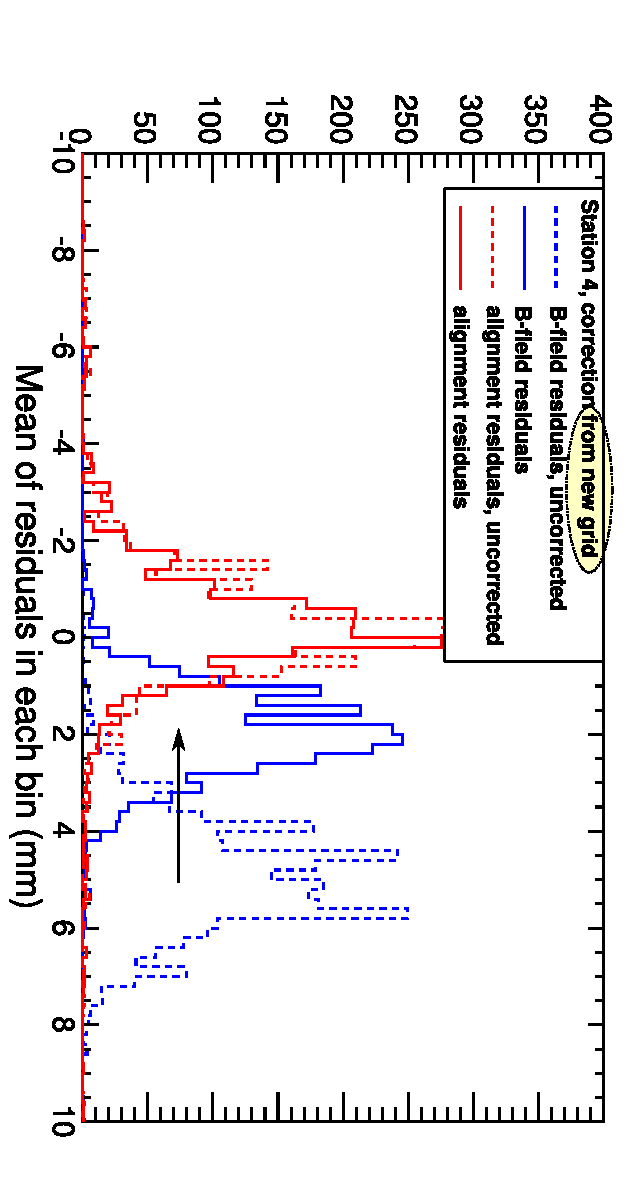
\includegraphics[width=4 cm, angle=90]{newgrid_corrections_station4.pdf} 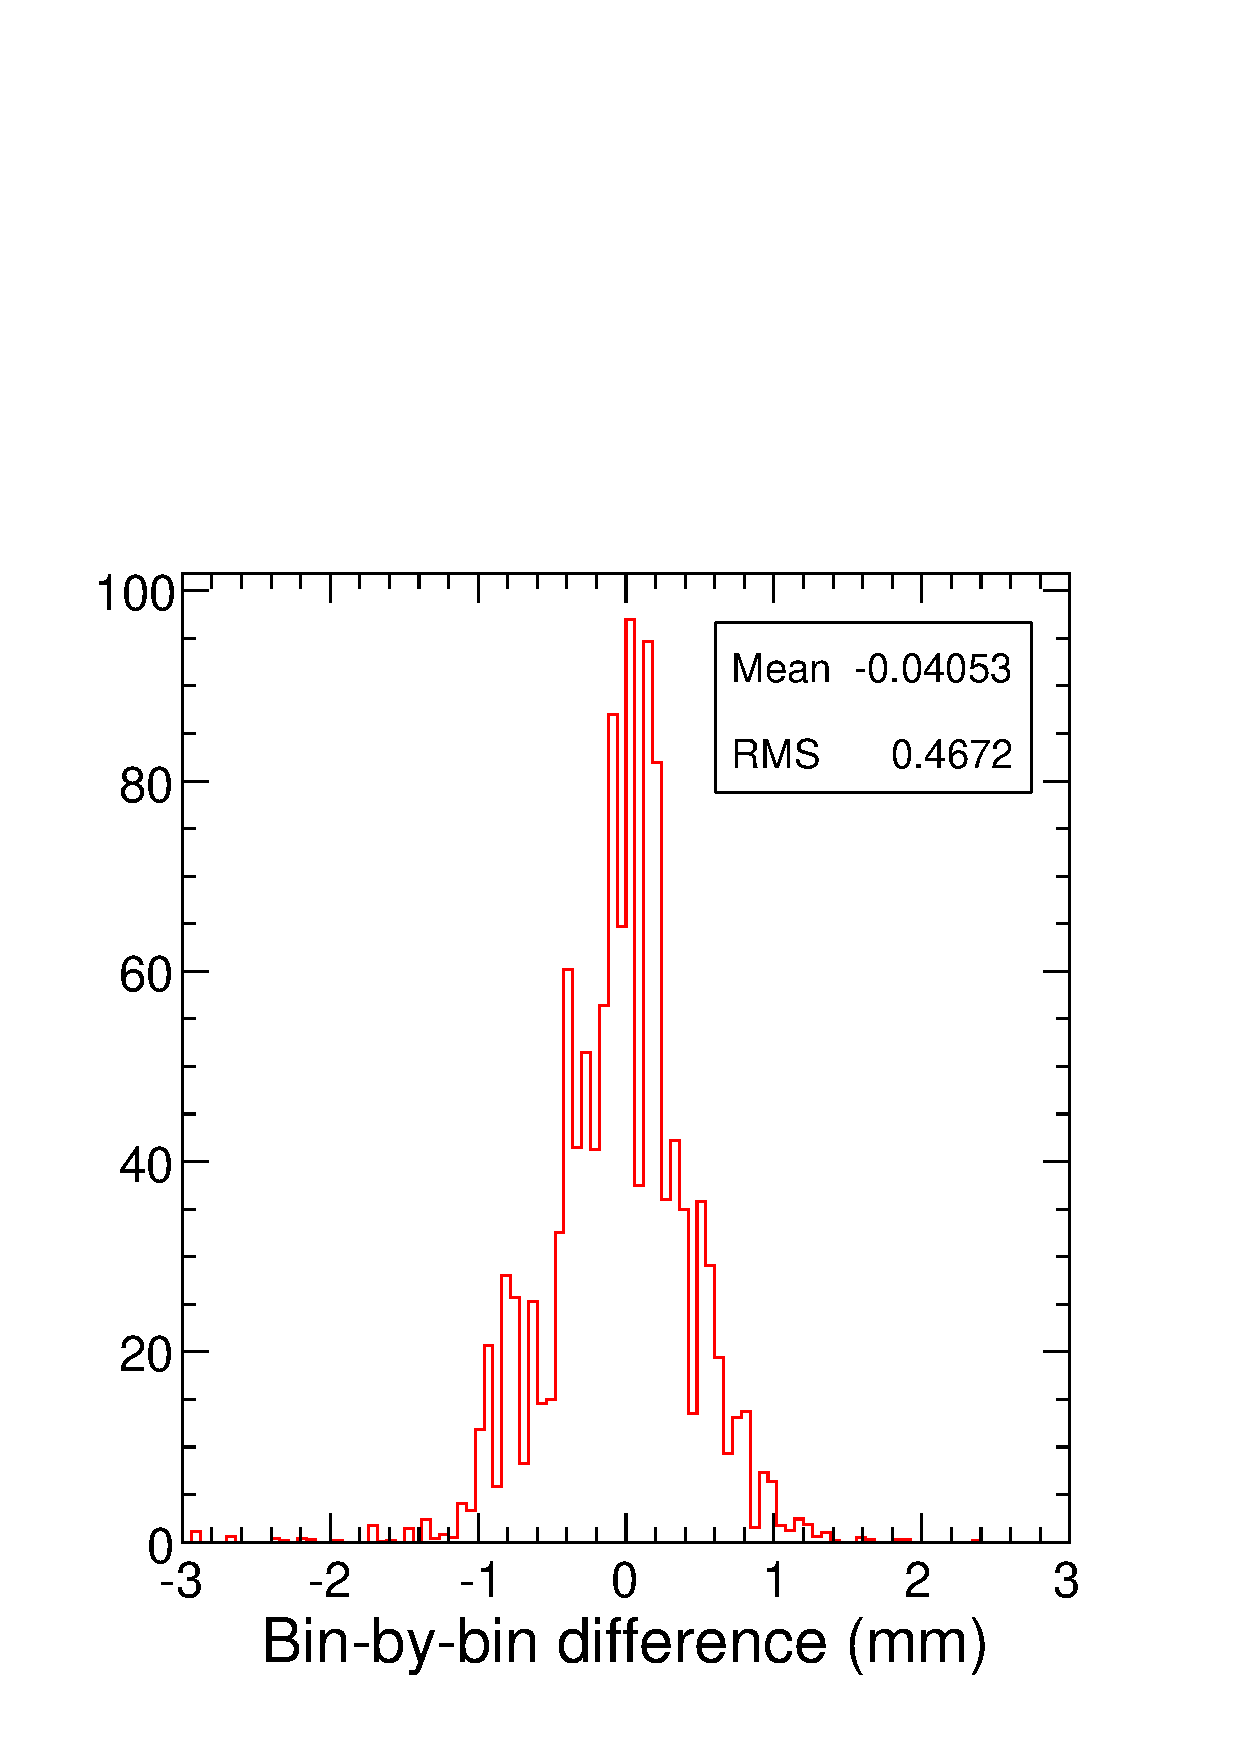
\includegraphics[height=4 cm]{newgrid_binbybin_station4.pdf}
\end{frame}

\begin{frame}
\frametitle{Sawtooth effect (1/2)}

\begin{columns}
\column{0.5\linewidth}
\begin{itemize}
\item Alignment plots revealed $r\phi$ residual vs.~$\phi$ structure inside \mbox{chambers (right)\hspace{-1 cm}}
\item Entrance angle is correlated \mbox{with $\phi_{\mbox{\tiny global}}$\hspace{-0.5 cm}} (i.e.~$x$) and more relevant \mbox{for chambers;\hspace{-1 cm}}
\textcolor{red}{correlation in data} is \mbox{stronger (below)\hspace{-1 cm}}
\item \textcolor{blue}{Collisions MC} doesn't \mbox{show the effect\hspace{-0.5 cm}} (shows a radial
  displacement instead: confirmed in orthogonal residuals, a separate
  \mbox{problem involving the propagator?)\hspace{-3 cm}}
\end{itemize}

\column{0.5\linewidth}
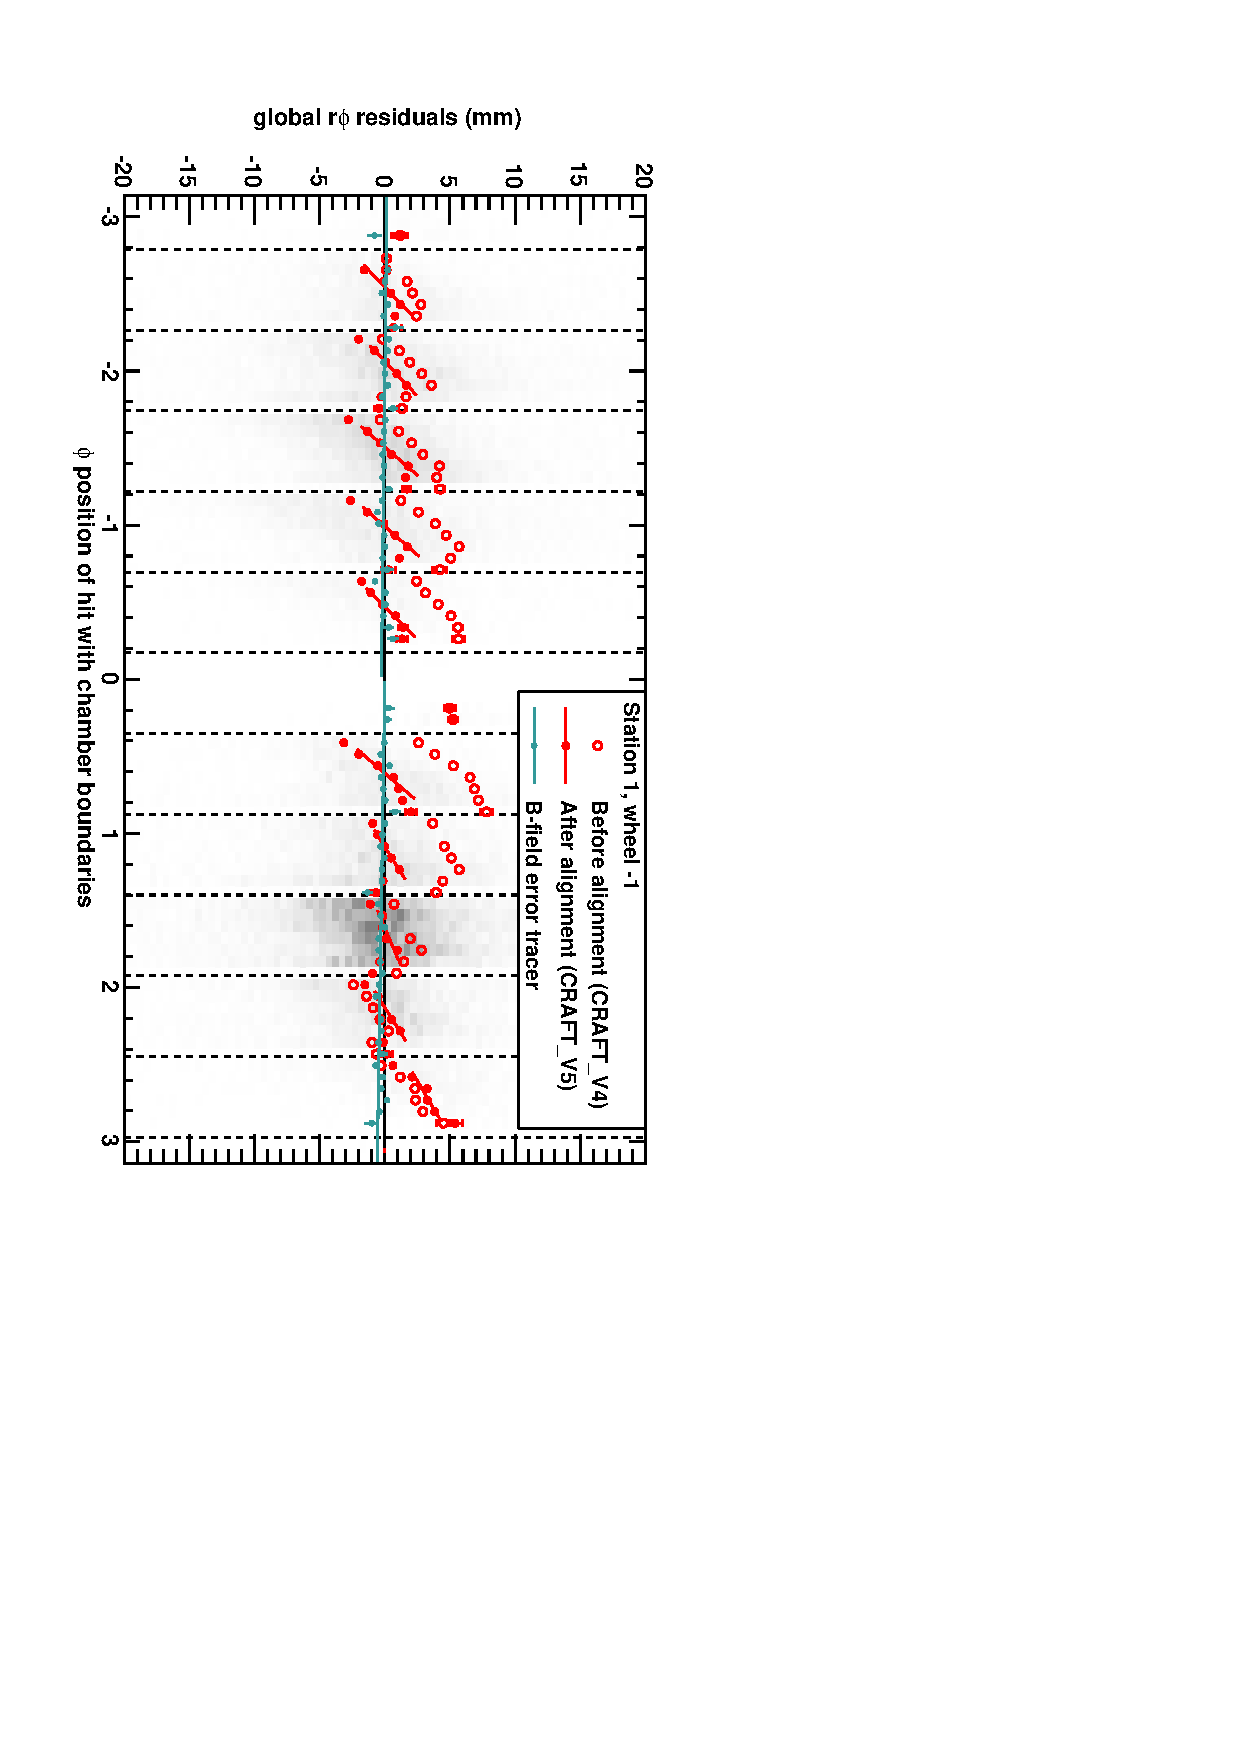
\includegraphics[height=\linewidth, angle=90]{alignmentplots_example2.pdf}
\end{columns}

\begin{center}
Focus on just one chamber (wheel 0, station 1, sector 10), $p_T > 40$~GeV

\mbox{ } \hfill 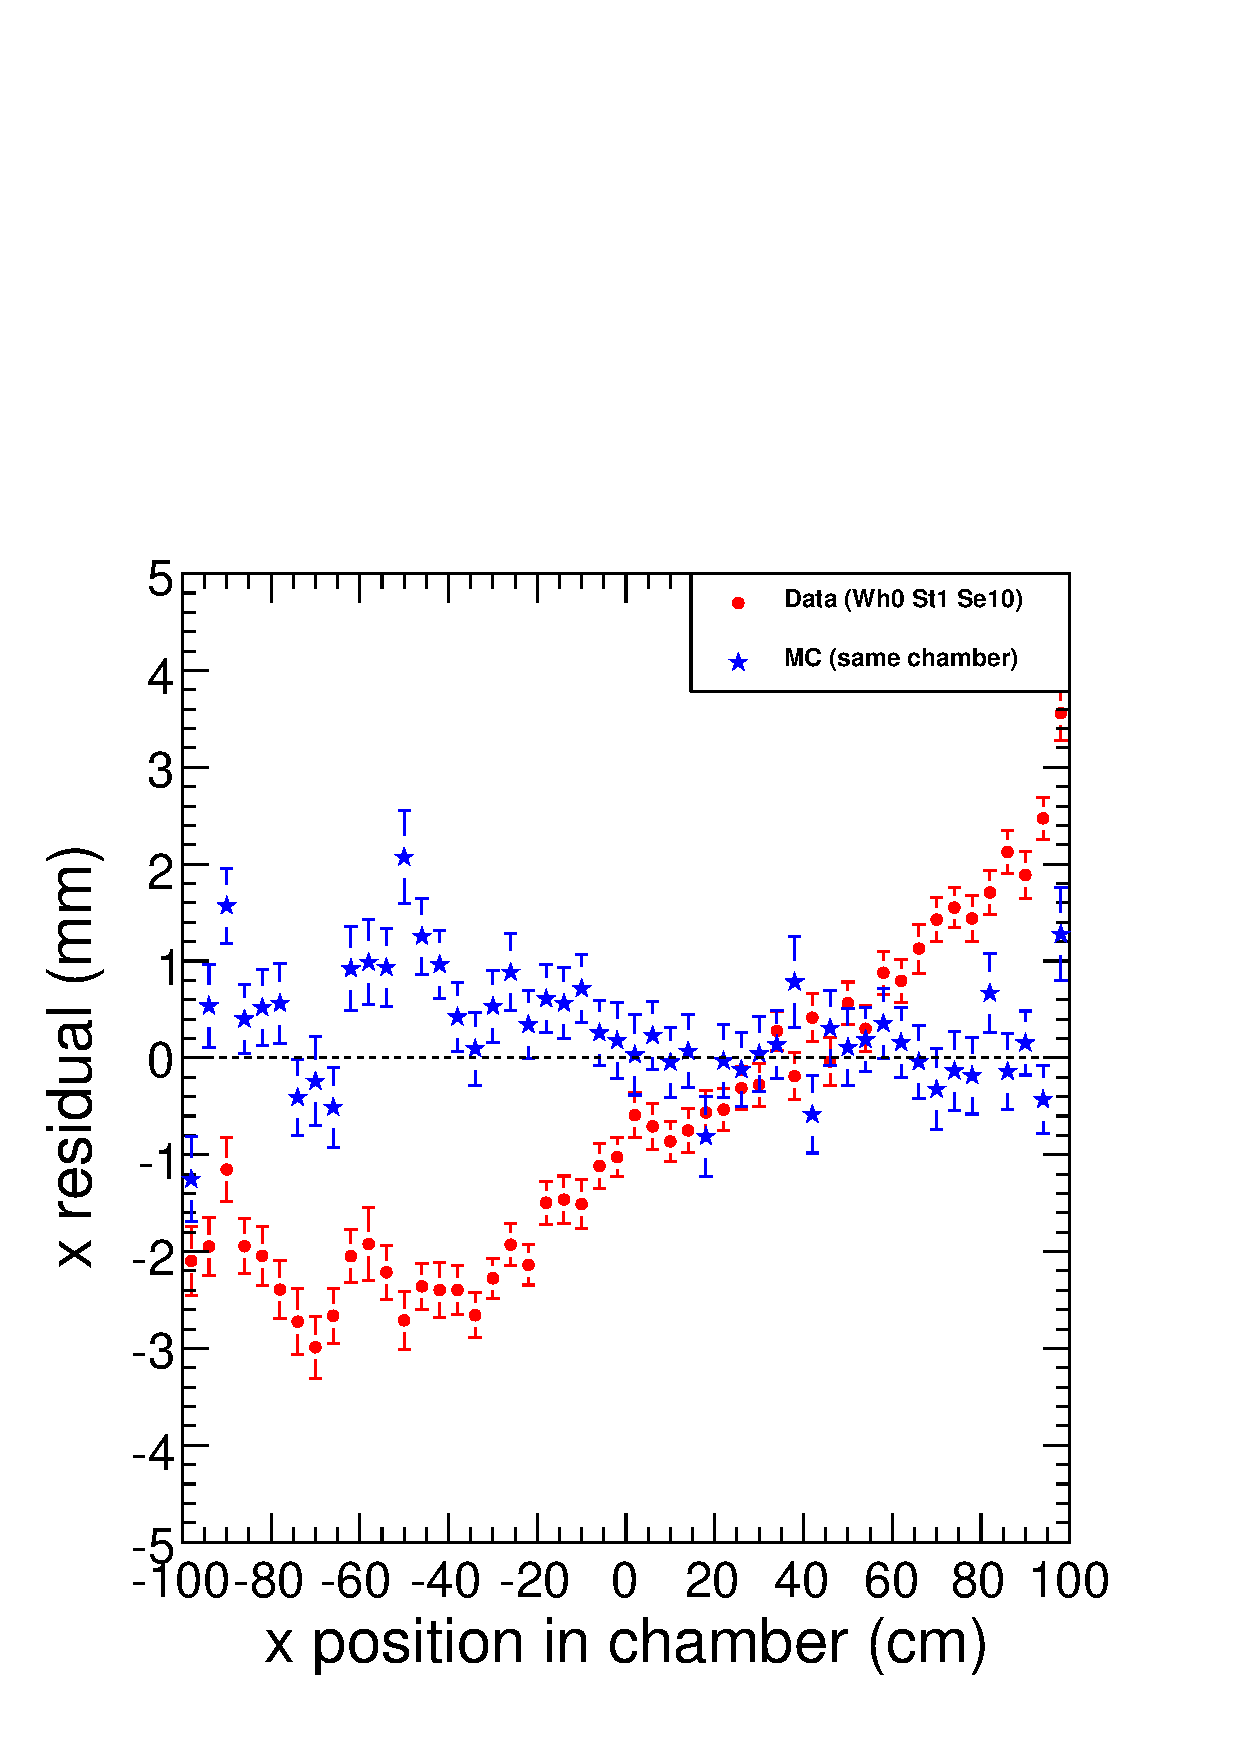
\includegraphics[width=0.37\linewidth]{original_sawtooth.pdf} \hfill 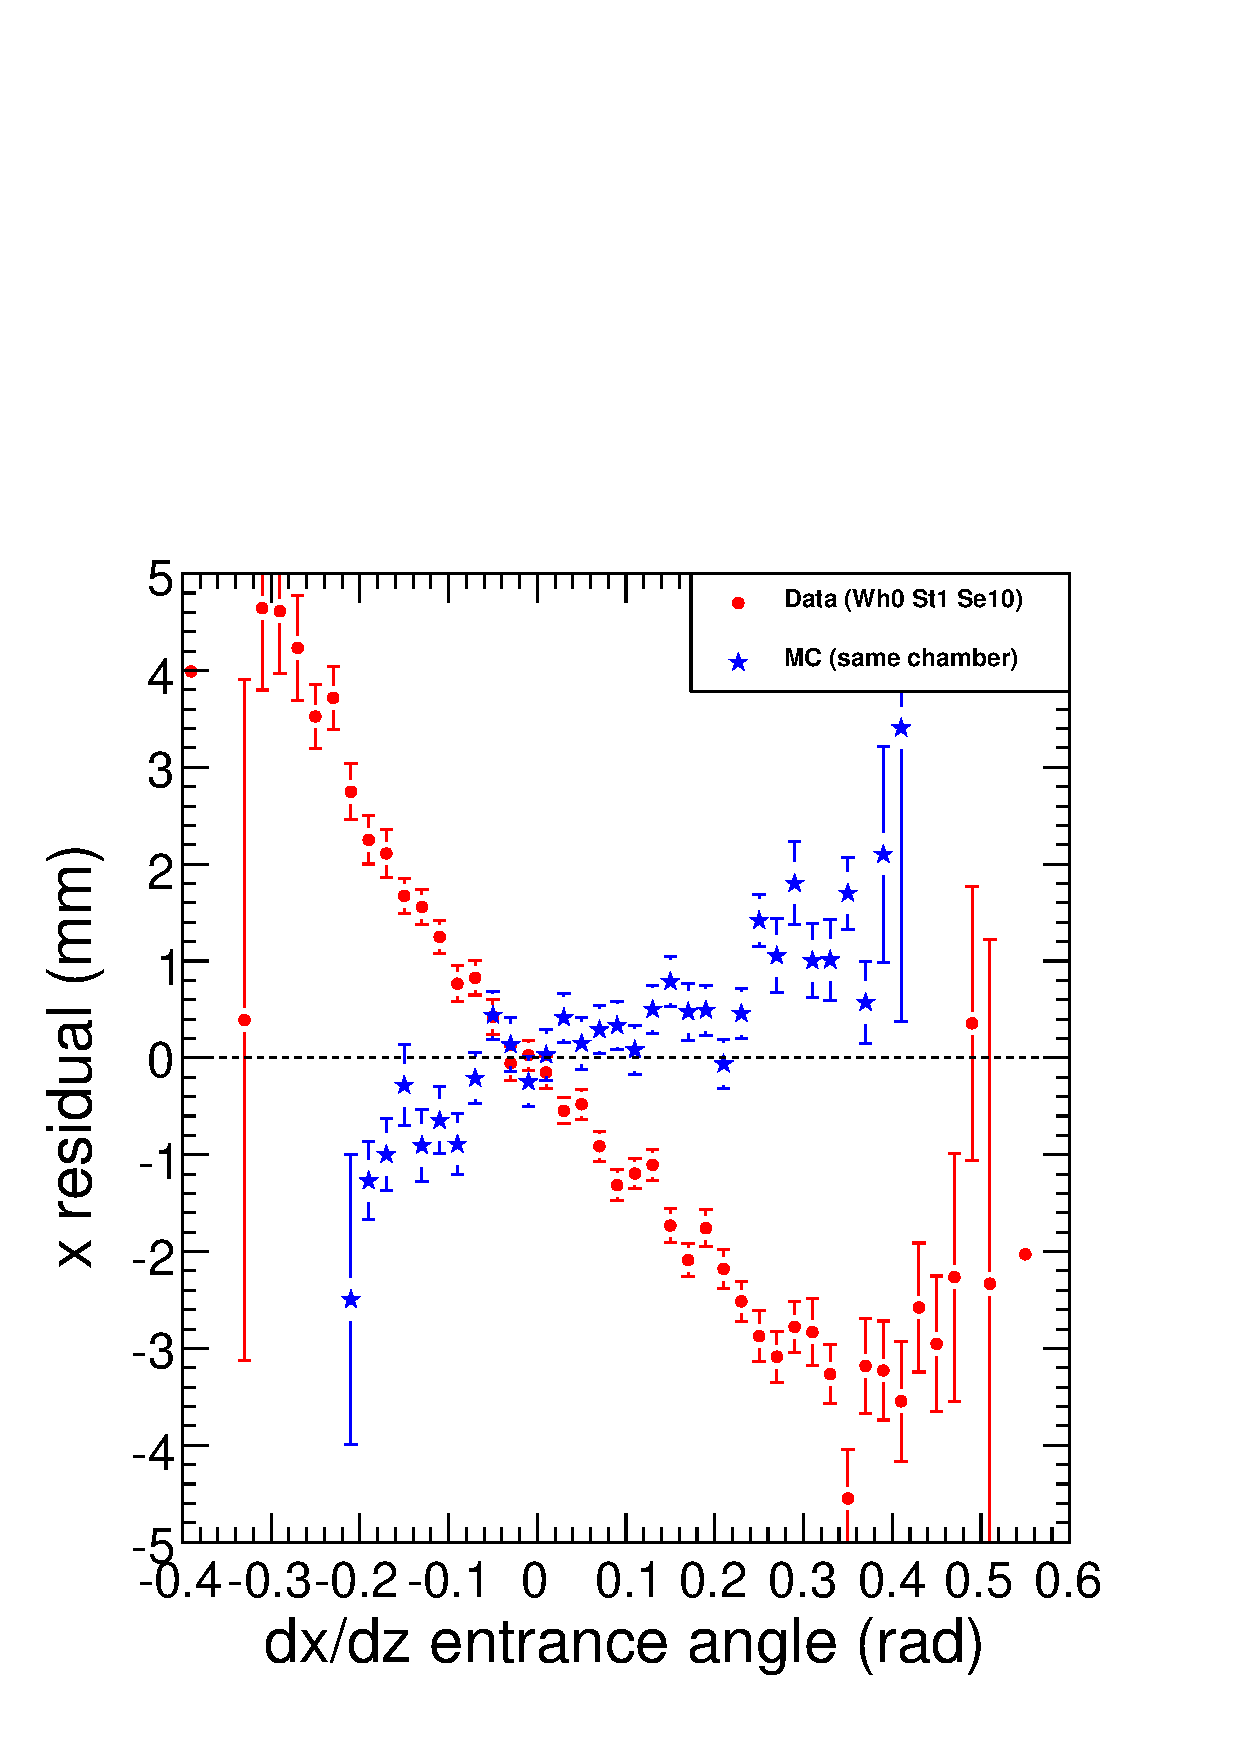
\includegraphics[width=0.37\linewidth]{vstrackangle_sawtooth.pdf} \hfill \begin{minipage}{1.6 cm} \vspace{-3 cm} \tiny data include latest $\vec{B}(\vec{x})$ map and superlayer radial corrections \end{minipage}\mbox{ }
\end{center}

\end{frame}

\begin{frame}
\frametitle{Sawtooth effect (2/2)}

\begin{columns}
\column{0.7\linewidth}
\begin{itemize}\setlength{\itemsep}{0.05 cm}
\item Seems to derive from an understandable effect: \mbox{$x$ residuals\hspace{-1 cm}}
  {\it should} be correlated with track-segment \mbox{angle difference\hspace{-1 cm}}
\item But an unexplained correlation between the \mbox{angle difference\hspace{-0.75 cm}} and
  the angle links $x$ residuals to angle \mbox{(sawtooth effect)\hspace{-1 cm}}
\item Second correlation is not understood and not in MC,

independent of $q$ and $p_T$ (unrelated to $\vec{B}$ and $dE/dx$)

\item Also, same effect in $y$ residuals vs.\ $dx/dz$ angle!

\item Ugo, Pablo, Alicia, and Paolo have started \mbox{investigating with segments and tracks\hspace{-5 cm}}

\end{itemize}

\column{0.3\linewidth}
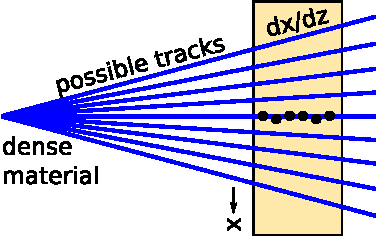
\includegraphics[width=\linewidth]{understandable_correlation_diagram.pdf}
\end{columns}

\vfill
\begin{columns}
\column{0.33\linewidth}
\mbox{ } \hfill \textcolor{darkblue}{this makes sense} \hfill \mbox{ }

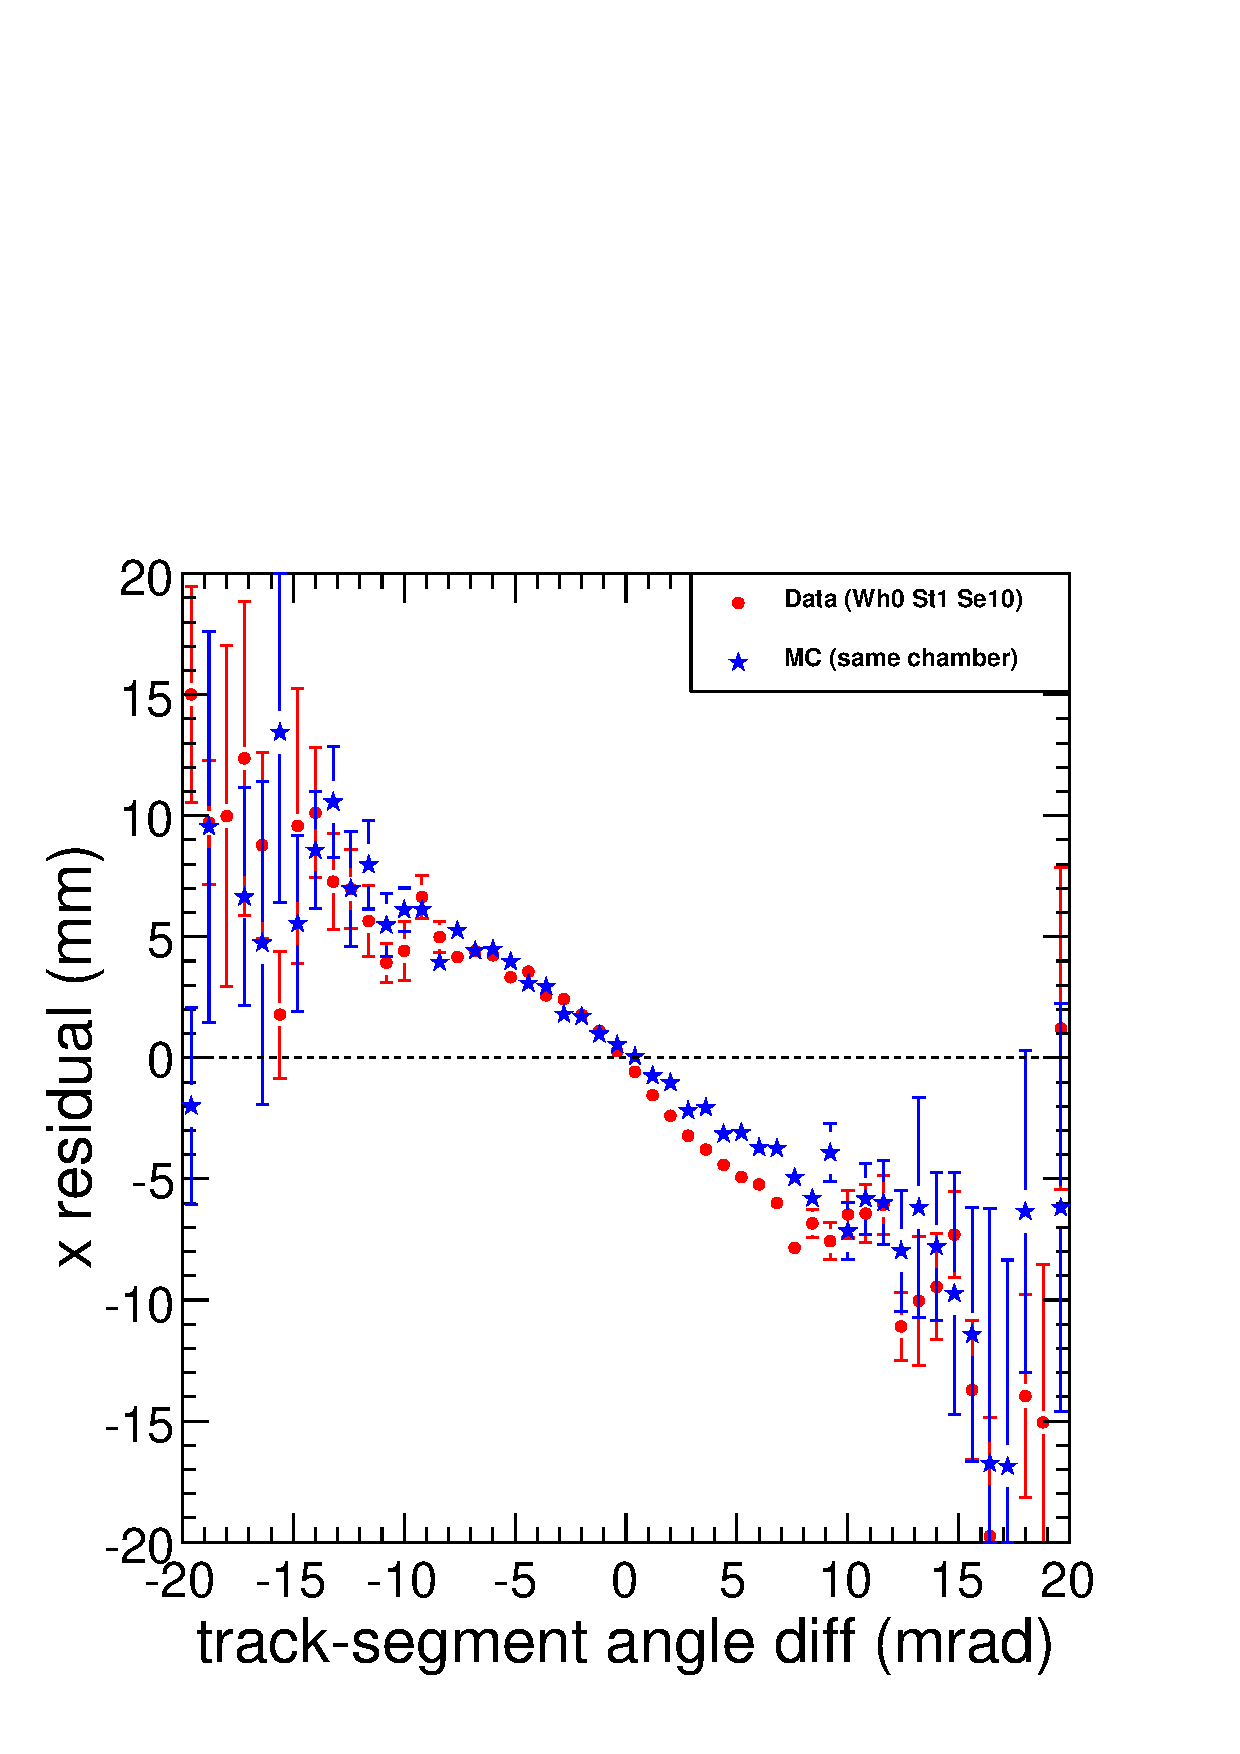
\includegraphics[width=\linewidth]{understandable_effect.pdf}

\column{0.33\linewidth}
\textcolor{darkblue}{why is this correlated \mbox{in data?\hspace{-1 cm}}}

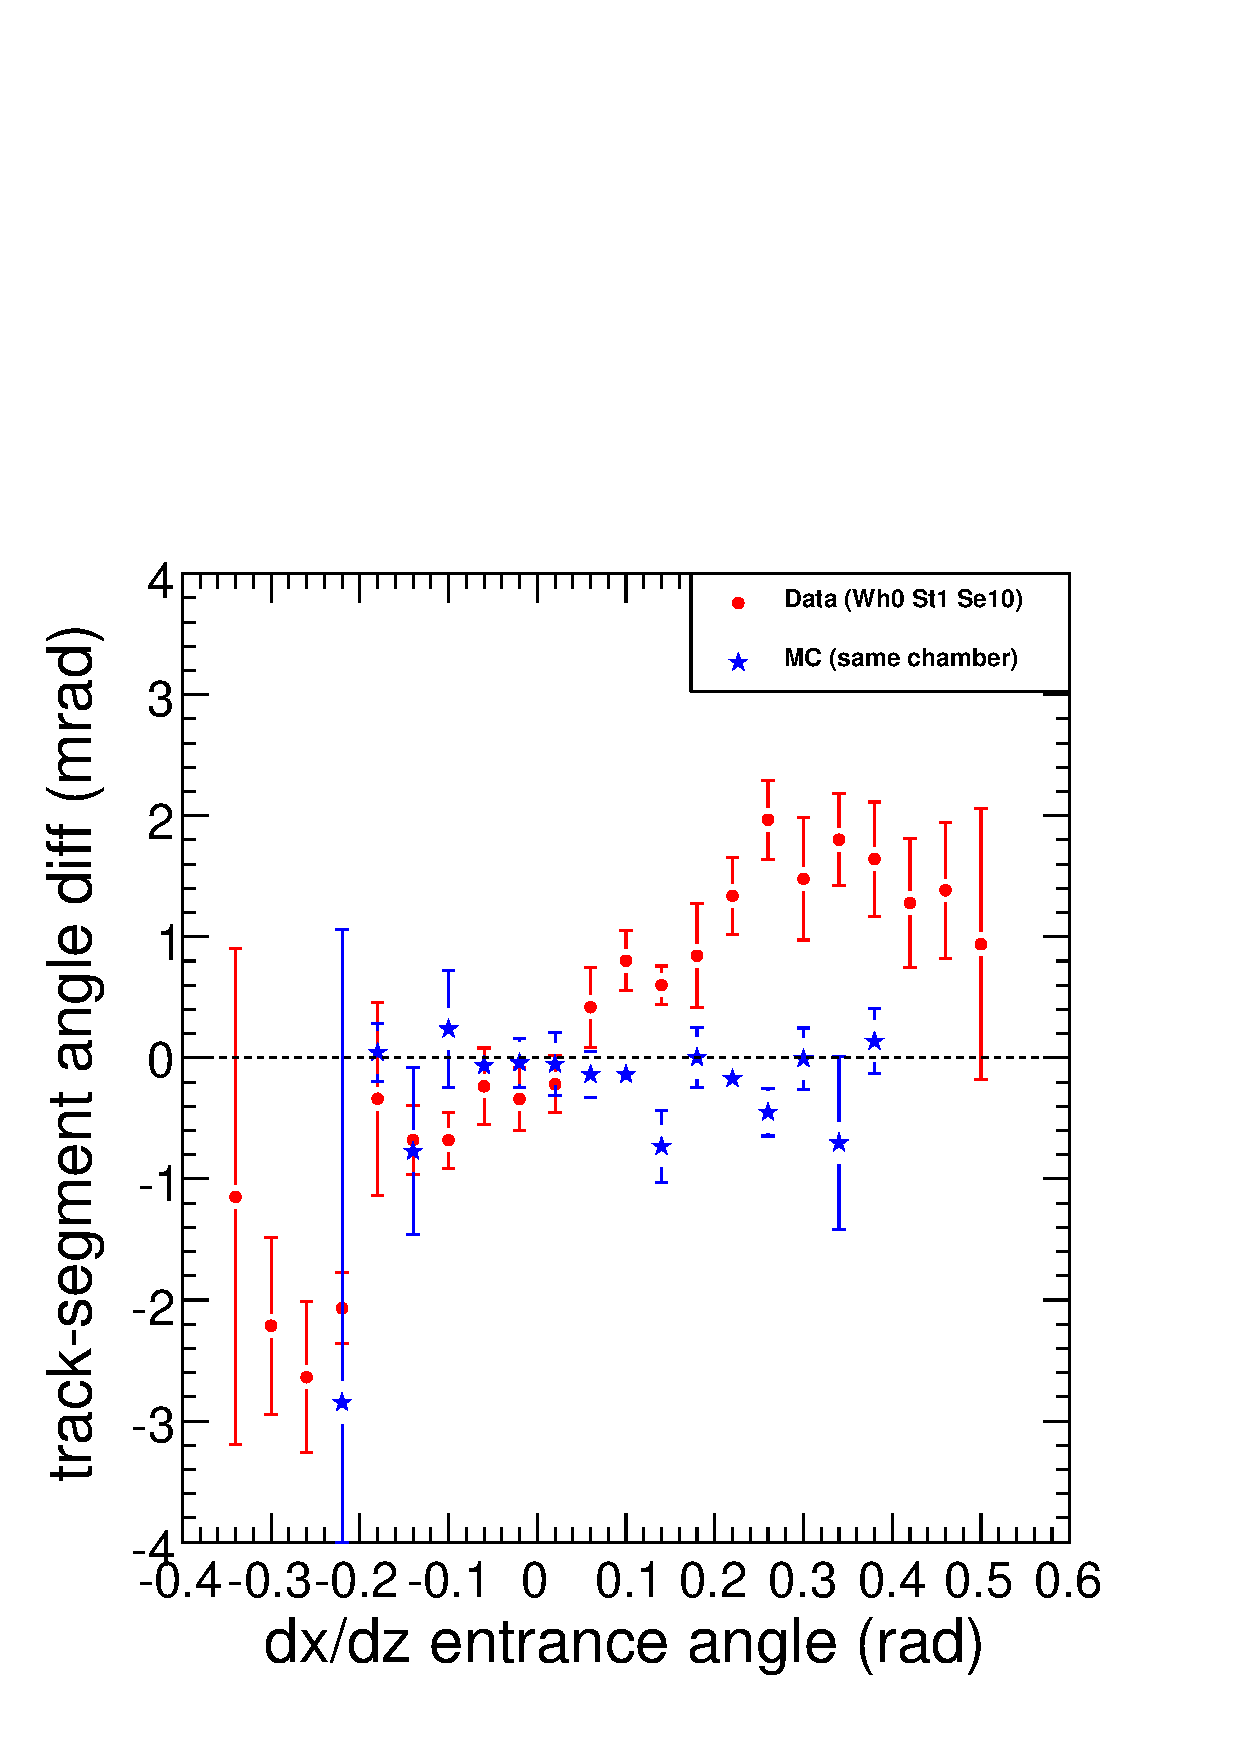
\includegraphics[width=\linewidth]{strange_correlation.pdf}

\column{0.33\linewidth}
\hfill \textcolor{darkblue}{and why do we see same} \hspace{0.07 cm}

\hfill \textcolor{darkblue}{effect on other parameter?}

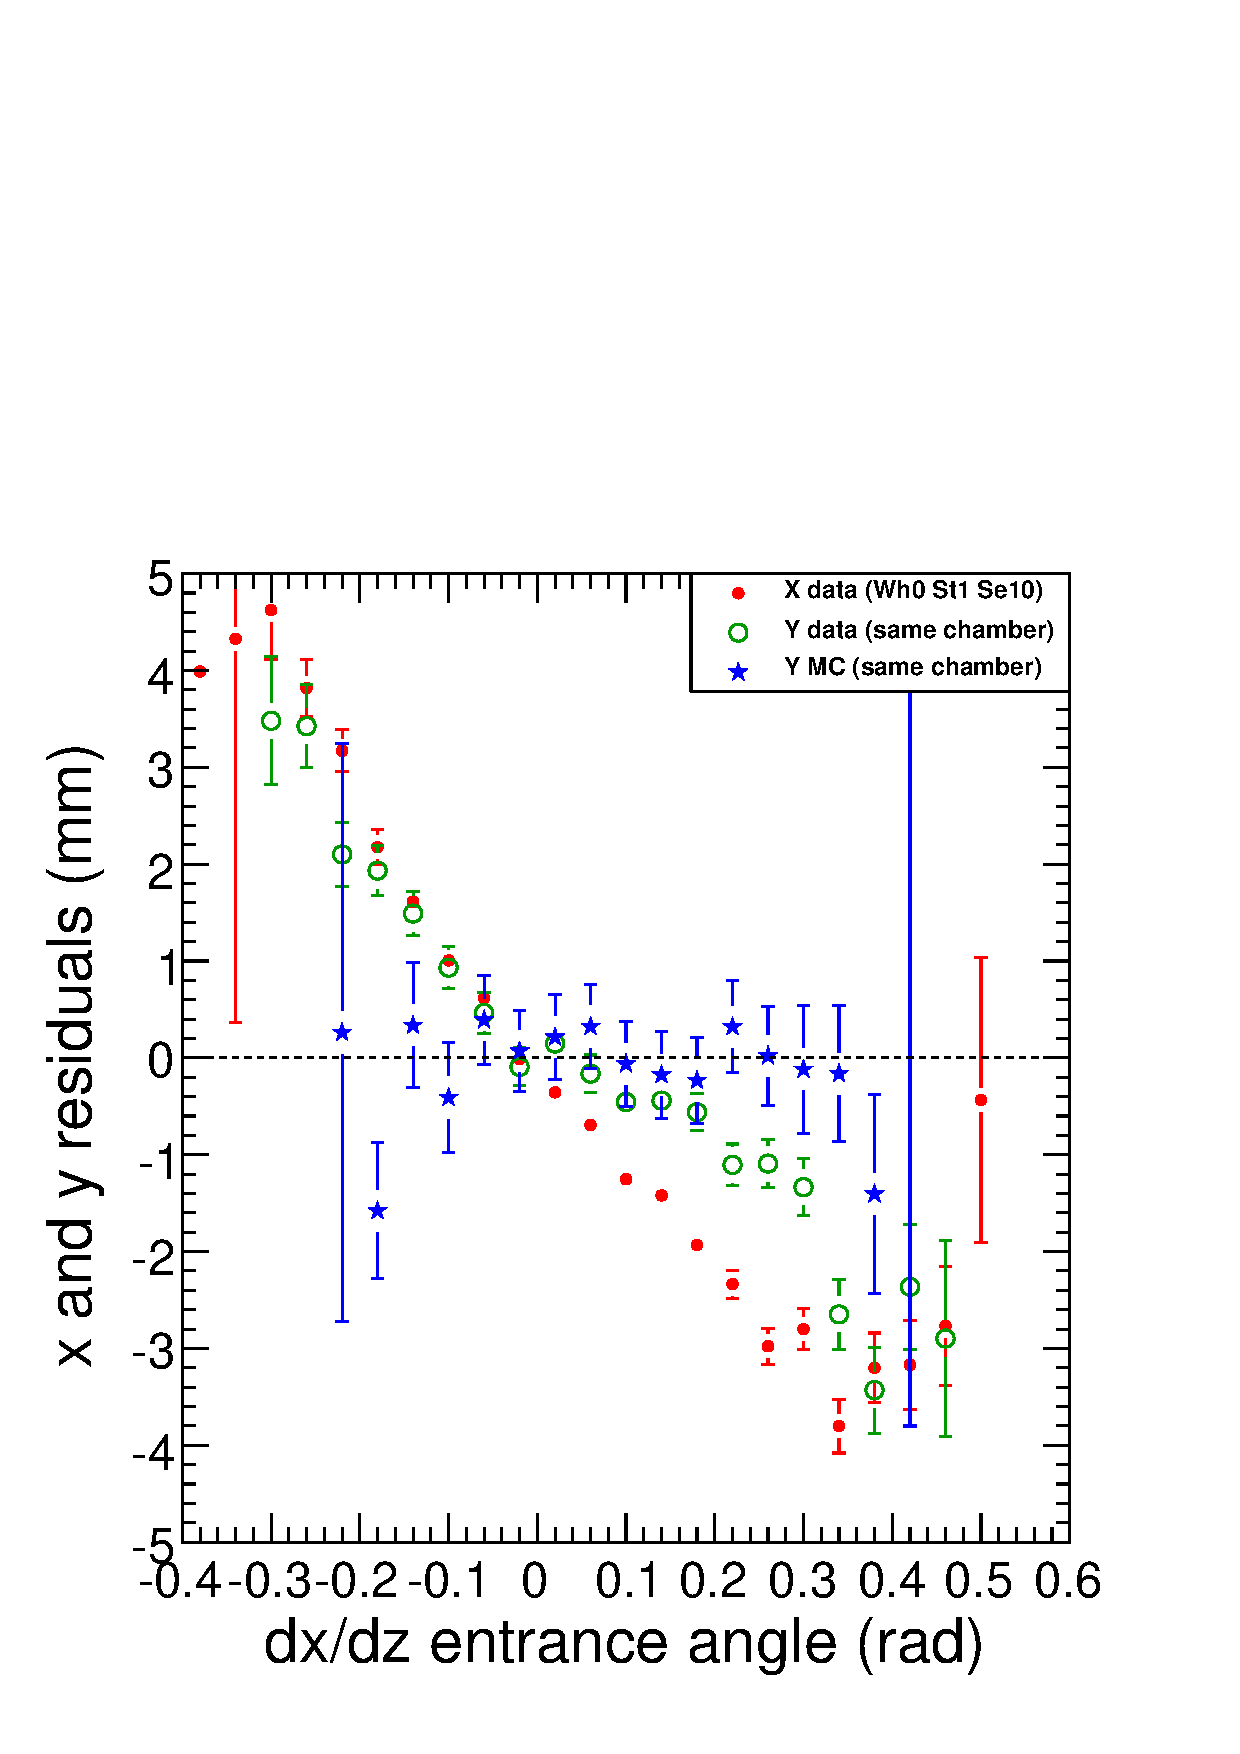
\includegraphics[width=\linewidth]{evenstranger_sawtooth.pdf}
\end{columns}
\end{frame}

\begin{frame}
\frametitle{Split globalMuon cosmics}

\begin{columns}
\column{0.65\linewidth}

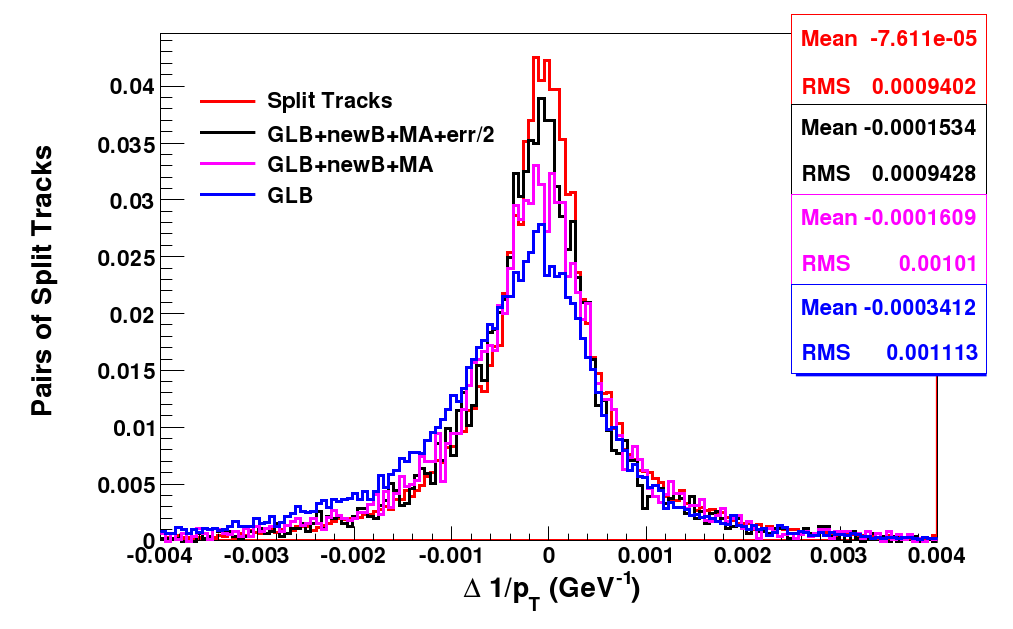
\includegraphics[width=\linewidth]{globalMuons_fixed.png}

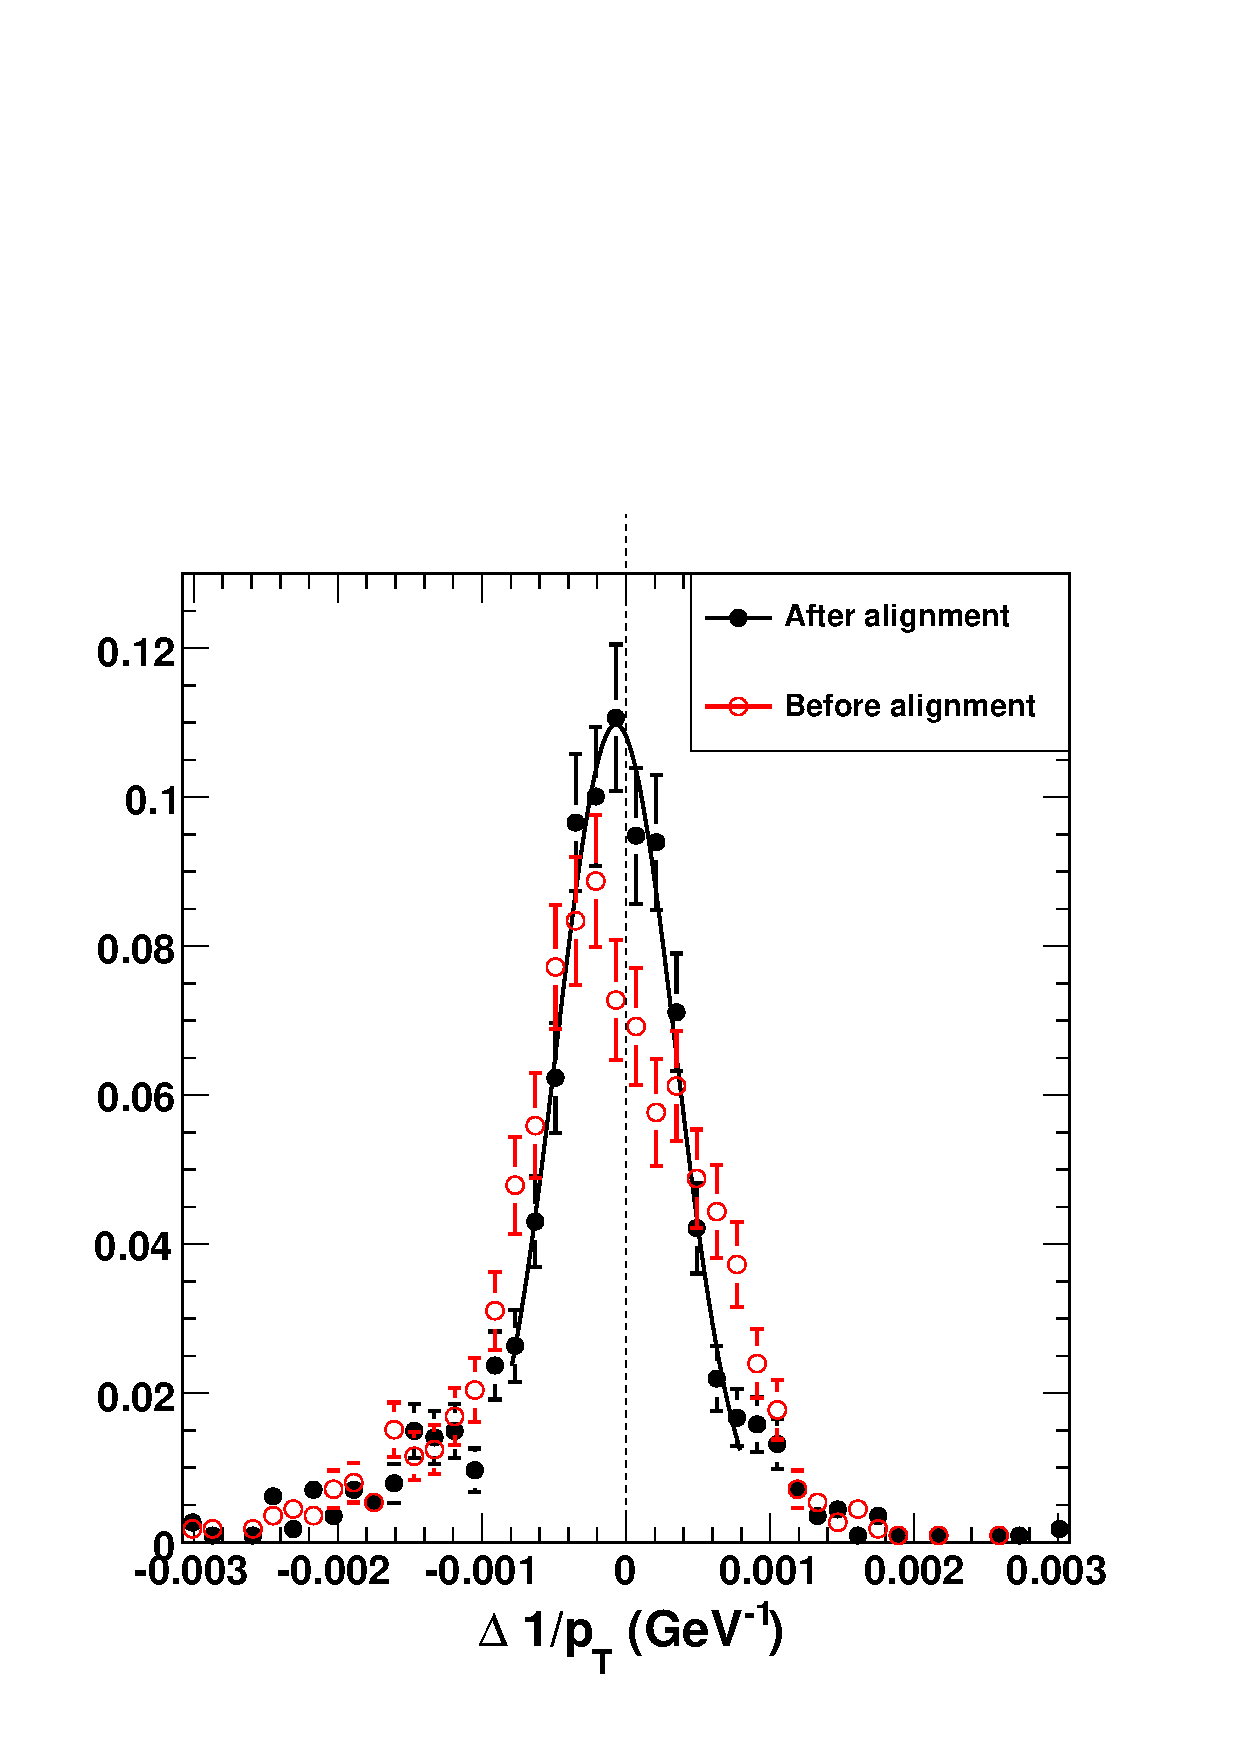
\includegraphics[width=0.5\linewidth]{delta_curv.pdf} 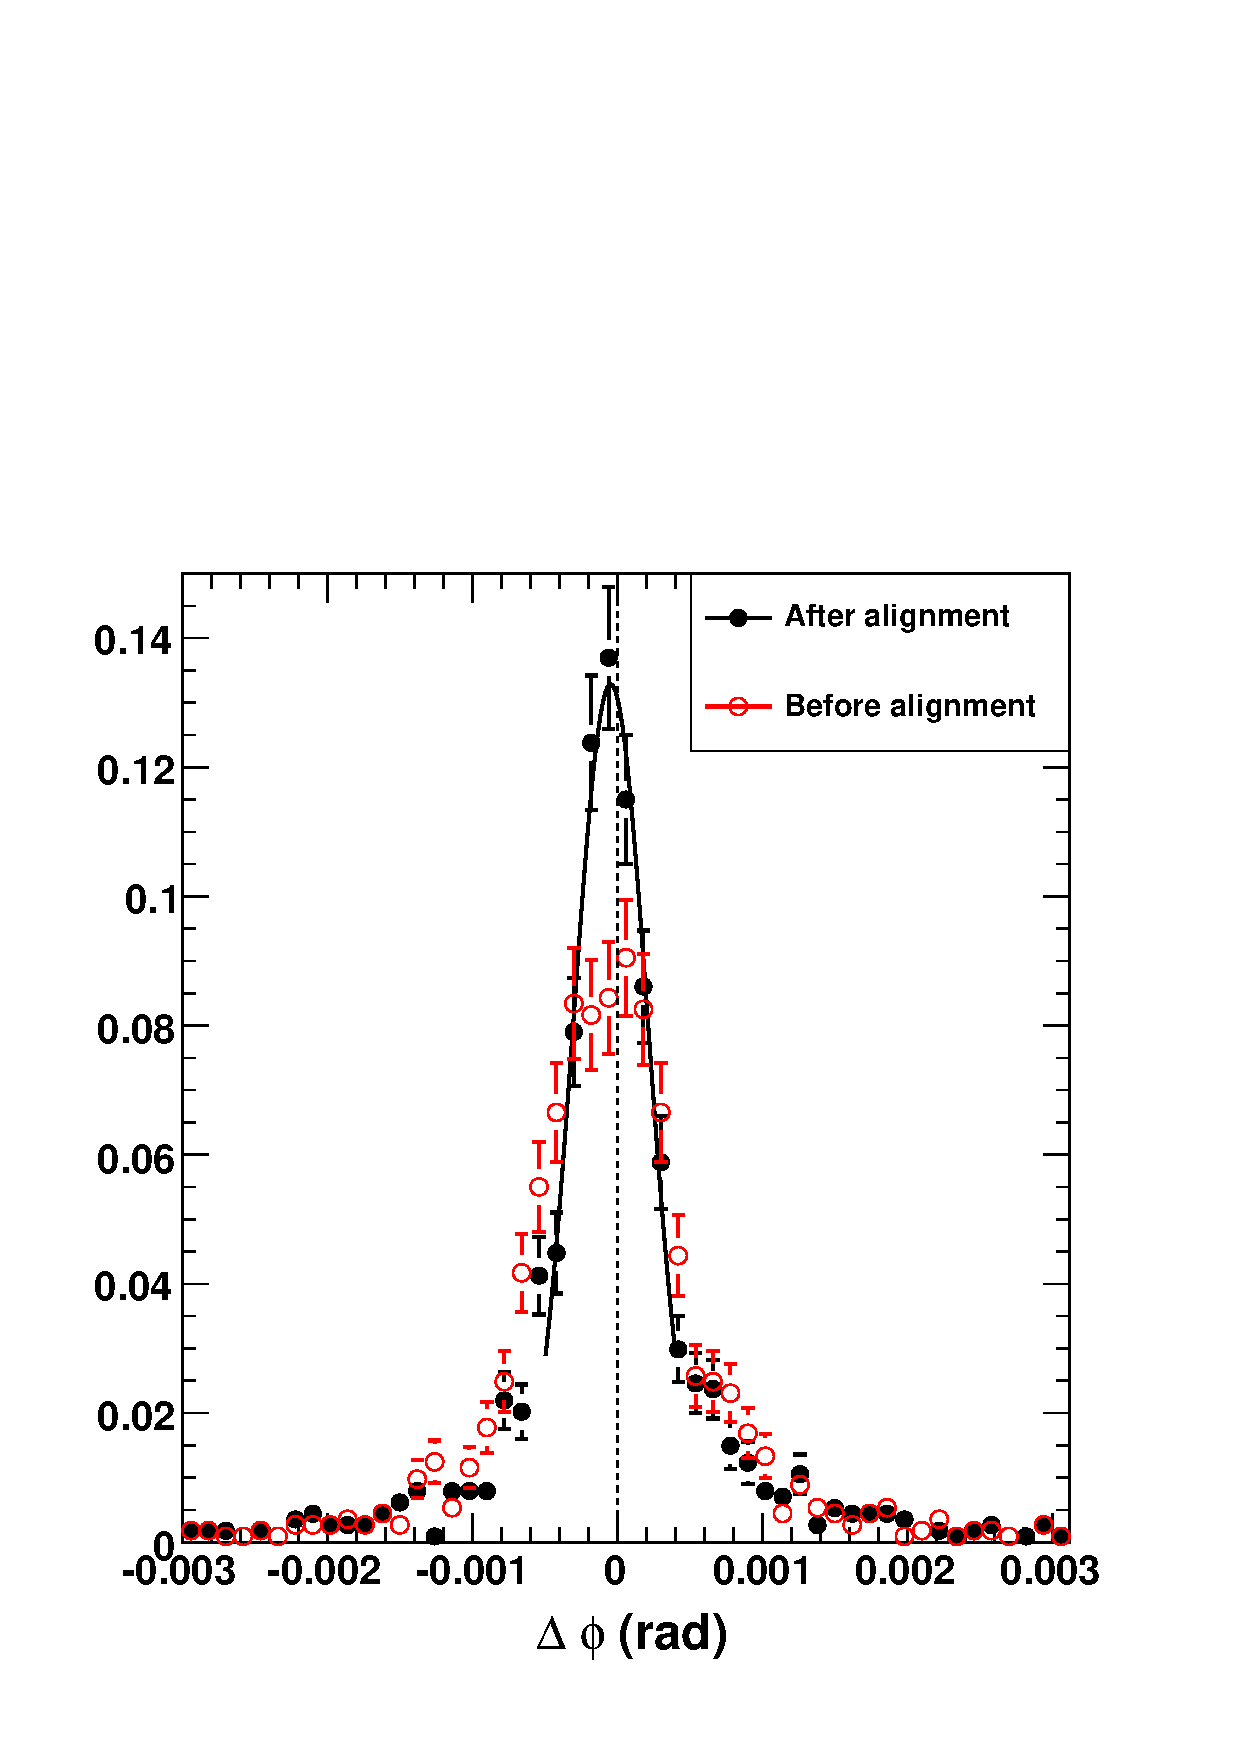
\includegraphics[width=0.5\linewidth]{delta_phi.pdf}

\column{0.4\linewidth}

\begin{itemize}
\item Deterioration of \mbox{globalMuons\hspace{-0.5 cm}} \textcolor{blue}{(GLB)} relative to tracker only \textcolor{red}{(Split Tracks)} due to three factors:
\begin{itemize}
\item \scriptsize muon alignment
\item \scriptsize wrong $\vec{B}(\vec{x})$
\item \scriptsize overestimated tracker alignment errors
\end{itemize}

\item New globalMuons (black) almost reproduces tracker, as it's supposed to (MC is at this level of agreement)

\item Bottom two plots highlight the muon alignment part
\begin{itemize}
\item \scriptsize $p_T > 100$~GeV
\item \scriptsize stations 1\&2 only
\item \scriptsize muon alignment is the only change shown
\end{itemize}
\end{itemize}
\end{columns}
\end{frame}

\begin{frame}
\frametitle{Residuals from hits in the fit}
\begin{columns}
\column{0.5\linewidth}
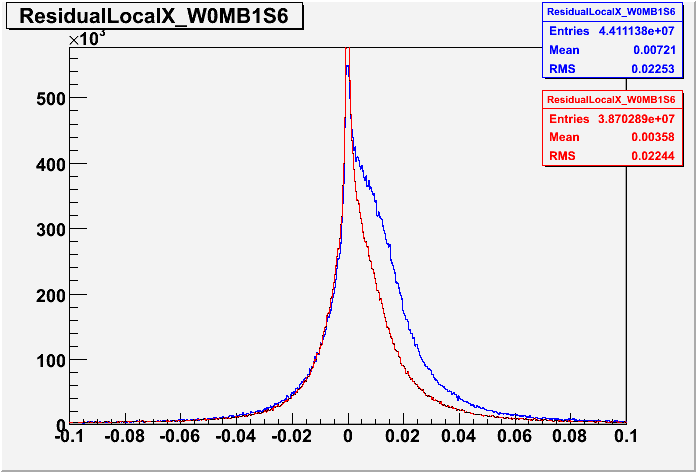
\includegraphics[width=\linewidth]{ResidualLocalX_W0MB1S6.png}

\vspace{0.75 cm}
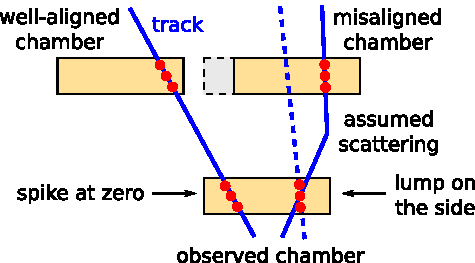
\includegraphics[width=\linewidth]{biased_residuals.pdf}

\column{0.5\linewidth}
\begin{itemize}
\item Muon residuals for hits included in the track-fit are complicated:
\begin{itemize}
\item \scriptsize non-Gaussian spike at zero from tracks biased toward hits
\item \scriptsize lump on the side from nearby misaligned chambers: segment is
  inconsistent with assumed scattering direction
\item \scriptsize long tails due to \mbox{real scattering\hspace{-1 cm}}
\end{itemize}
\item Mean and RMS do not characterize misalignment of observed
  chamber
\begin{itemize}
\item \scriptsize side-lumps related to other misalignments in neighborhood
\item \scriptsize definition of ``neighborhood'' depends strongly on distribution of tracks \\ (e.g.\ cosmics vs.\ LHC)
\item \scriptsize long tails hide lumps from RMS: 0.0224 vs.\ 0.0225 above
\item \scriptsize mean can be obscured by two lumps on either side
\end{itemize}
\end{itemize}

\end{columns}
\end{frame}

\begin{frame}
\frametitle{Current alignment incompleteness}

\begin{tabular}{c c}
\textcolor{darkblue}{Chambers aligned in $x$ and $\phi_z$} & \textcolor{darkblue}{Chambers aligned in $y$ (along beamline)} \\
& \\
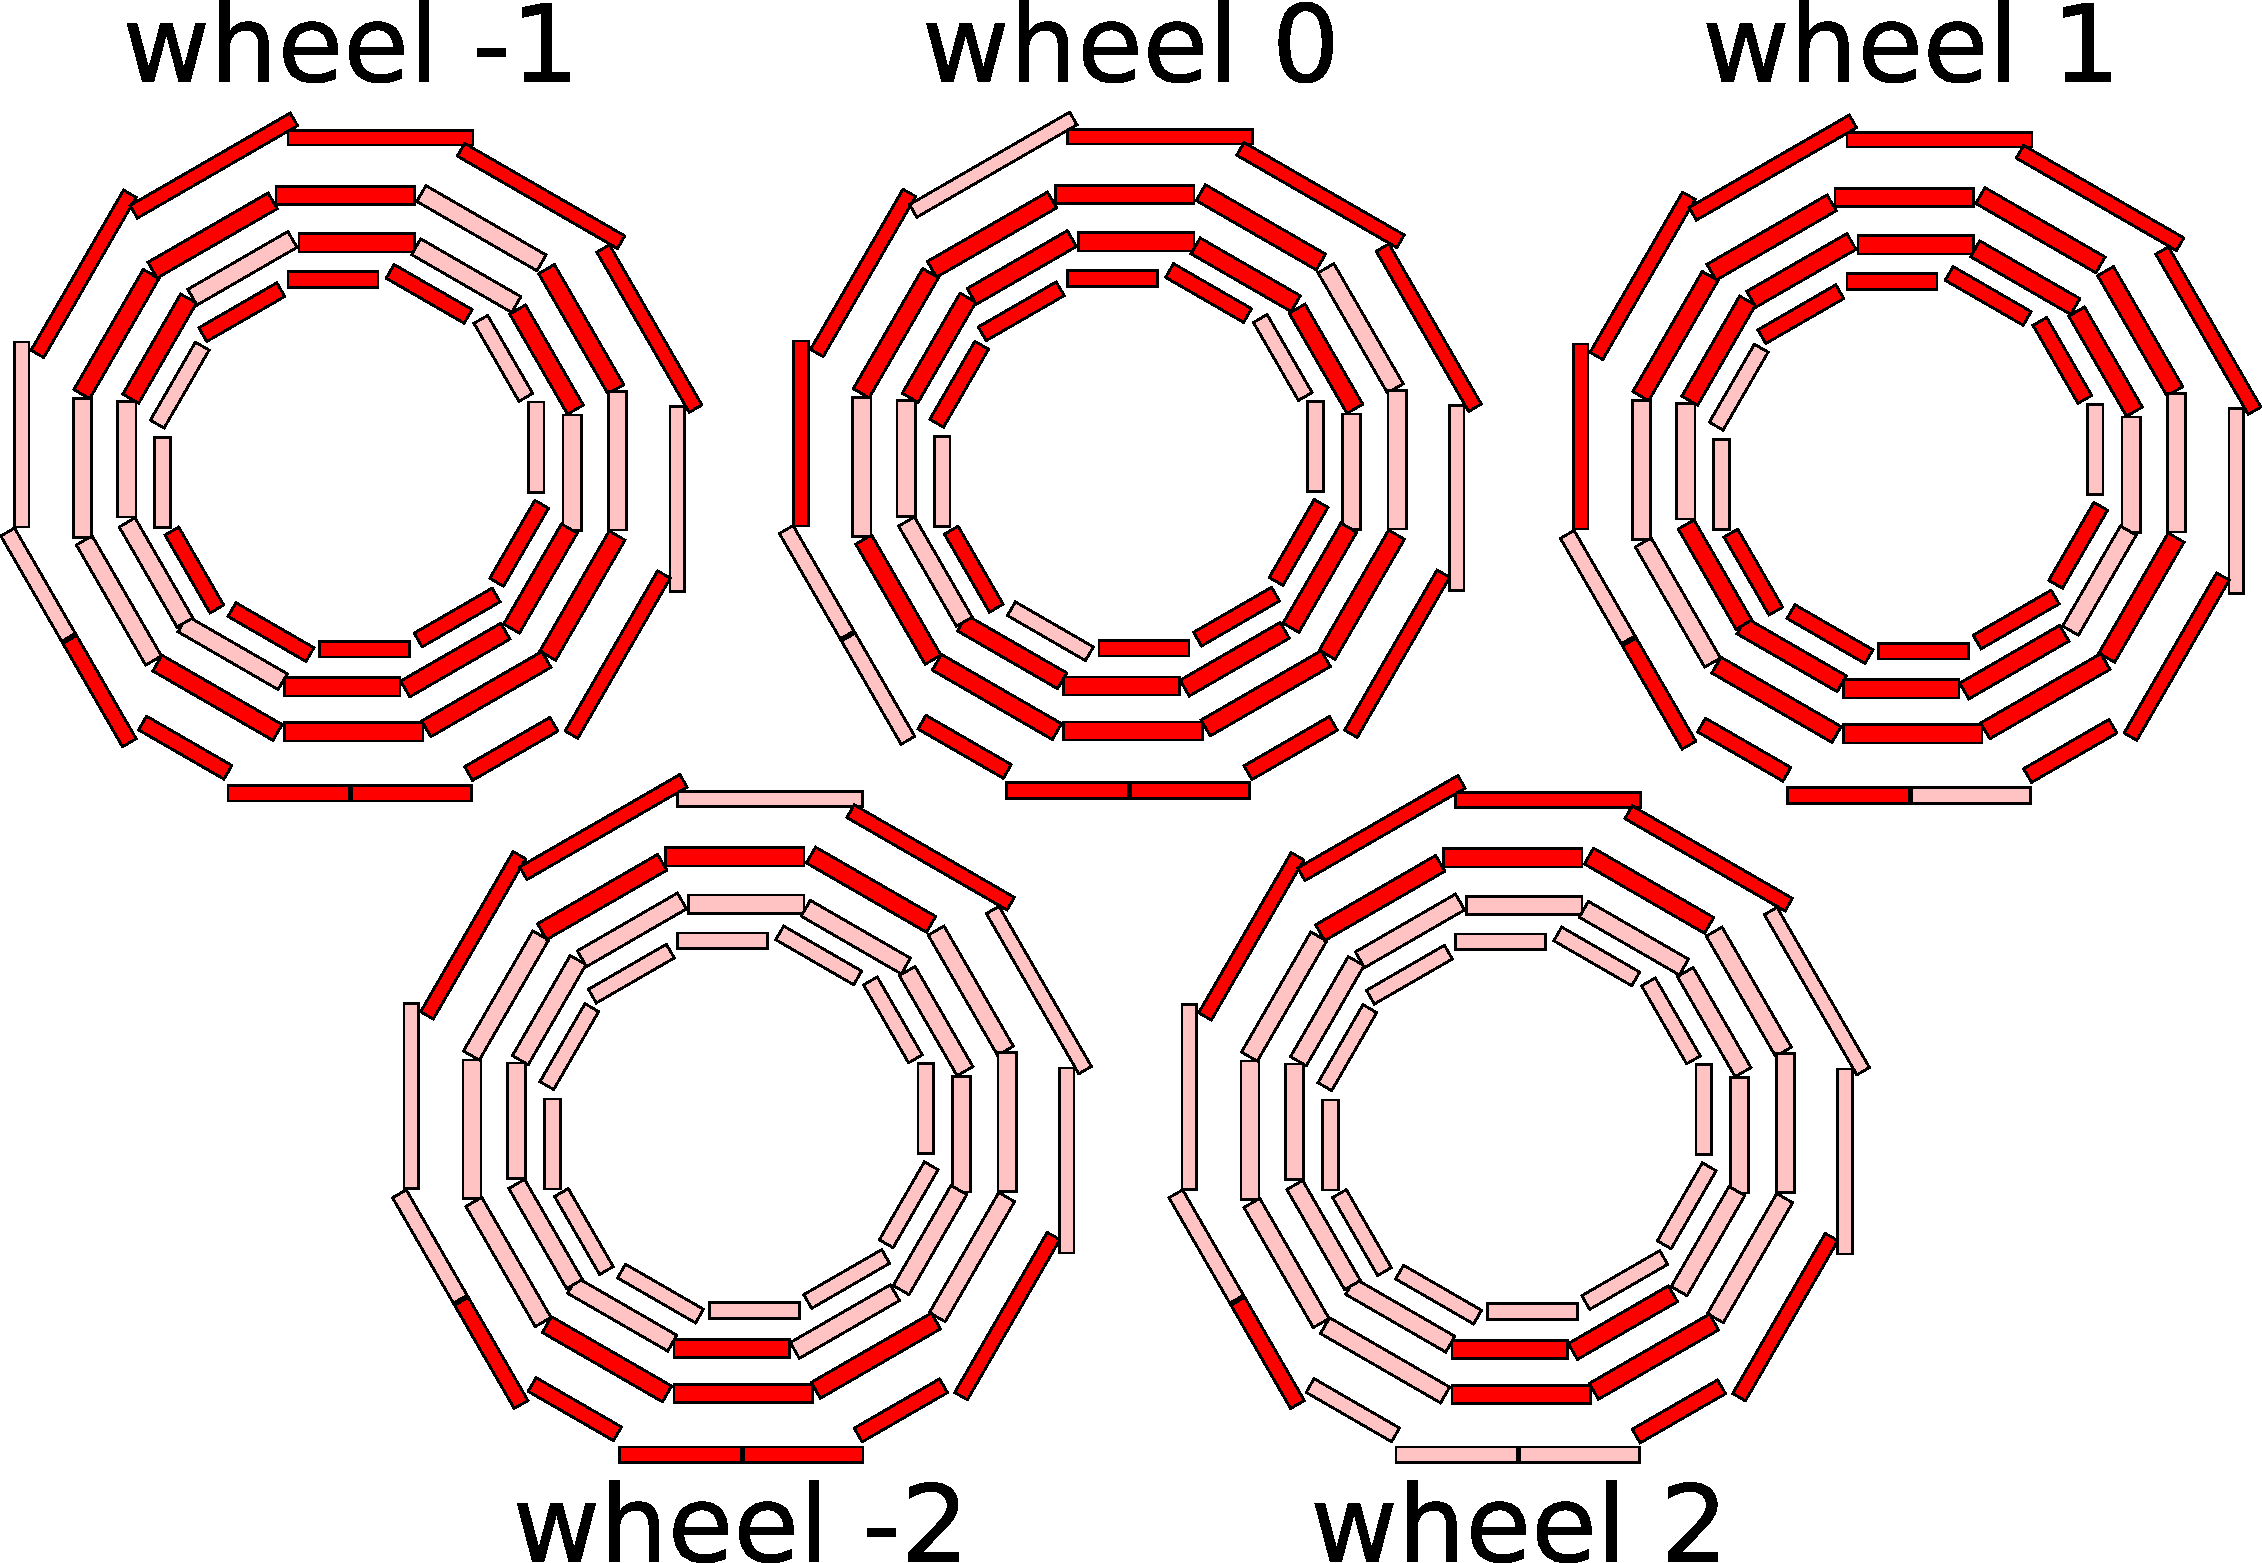
\includegraphics[width=0.45\linewidth]{aligned_rphi.pdf} & 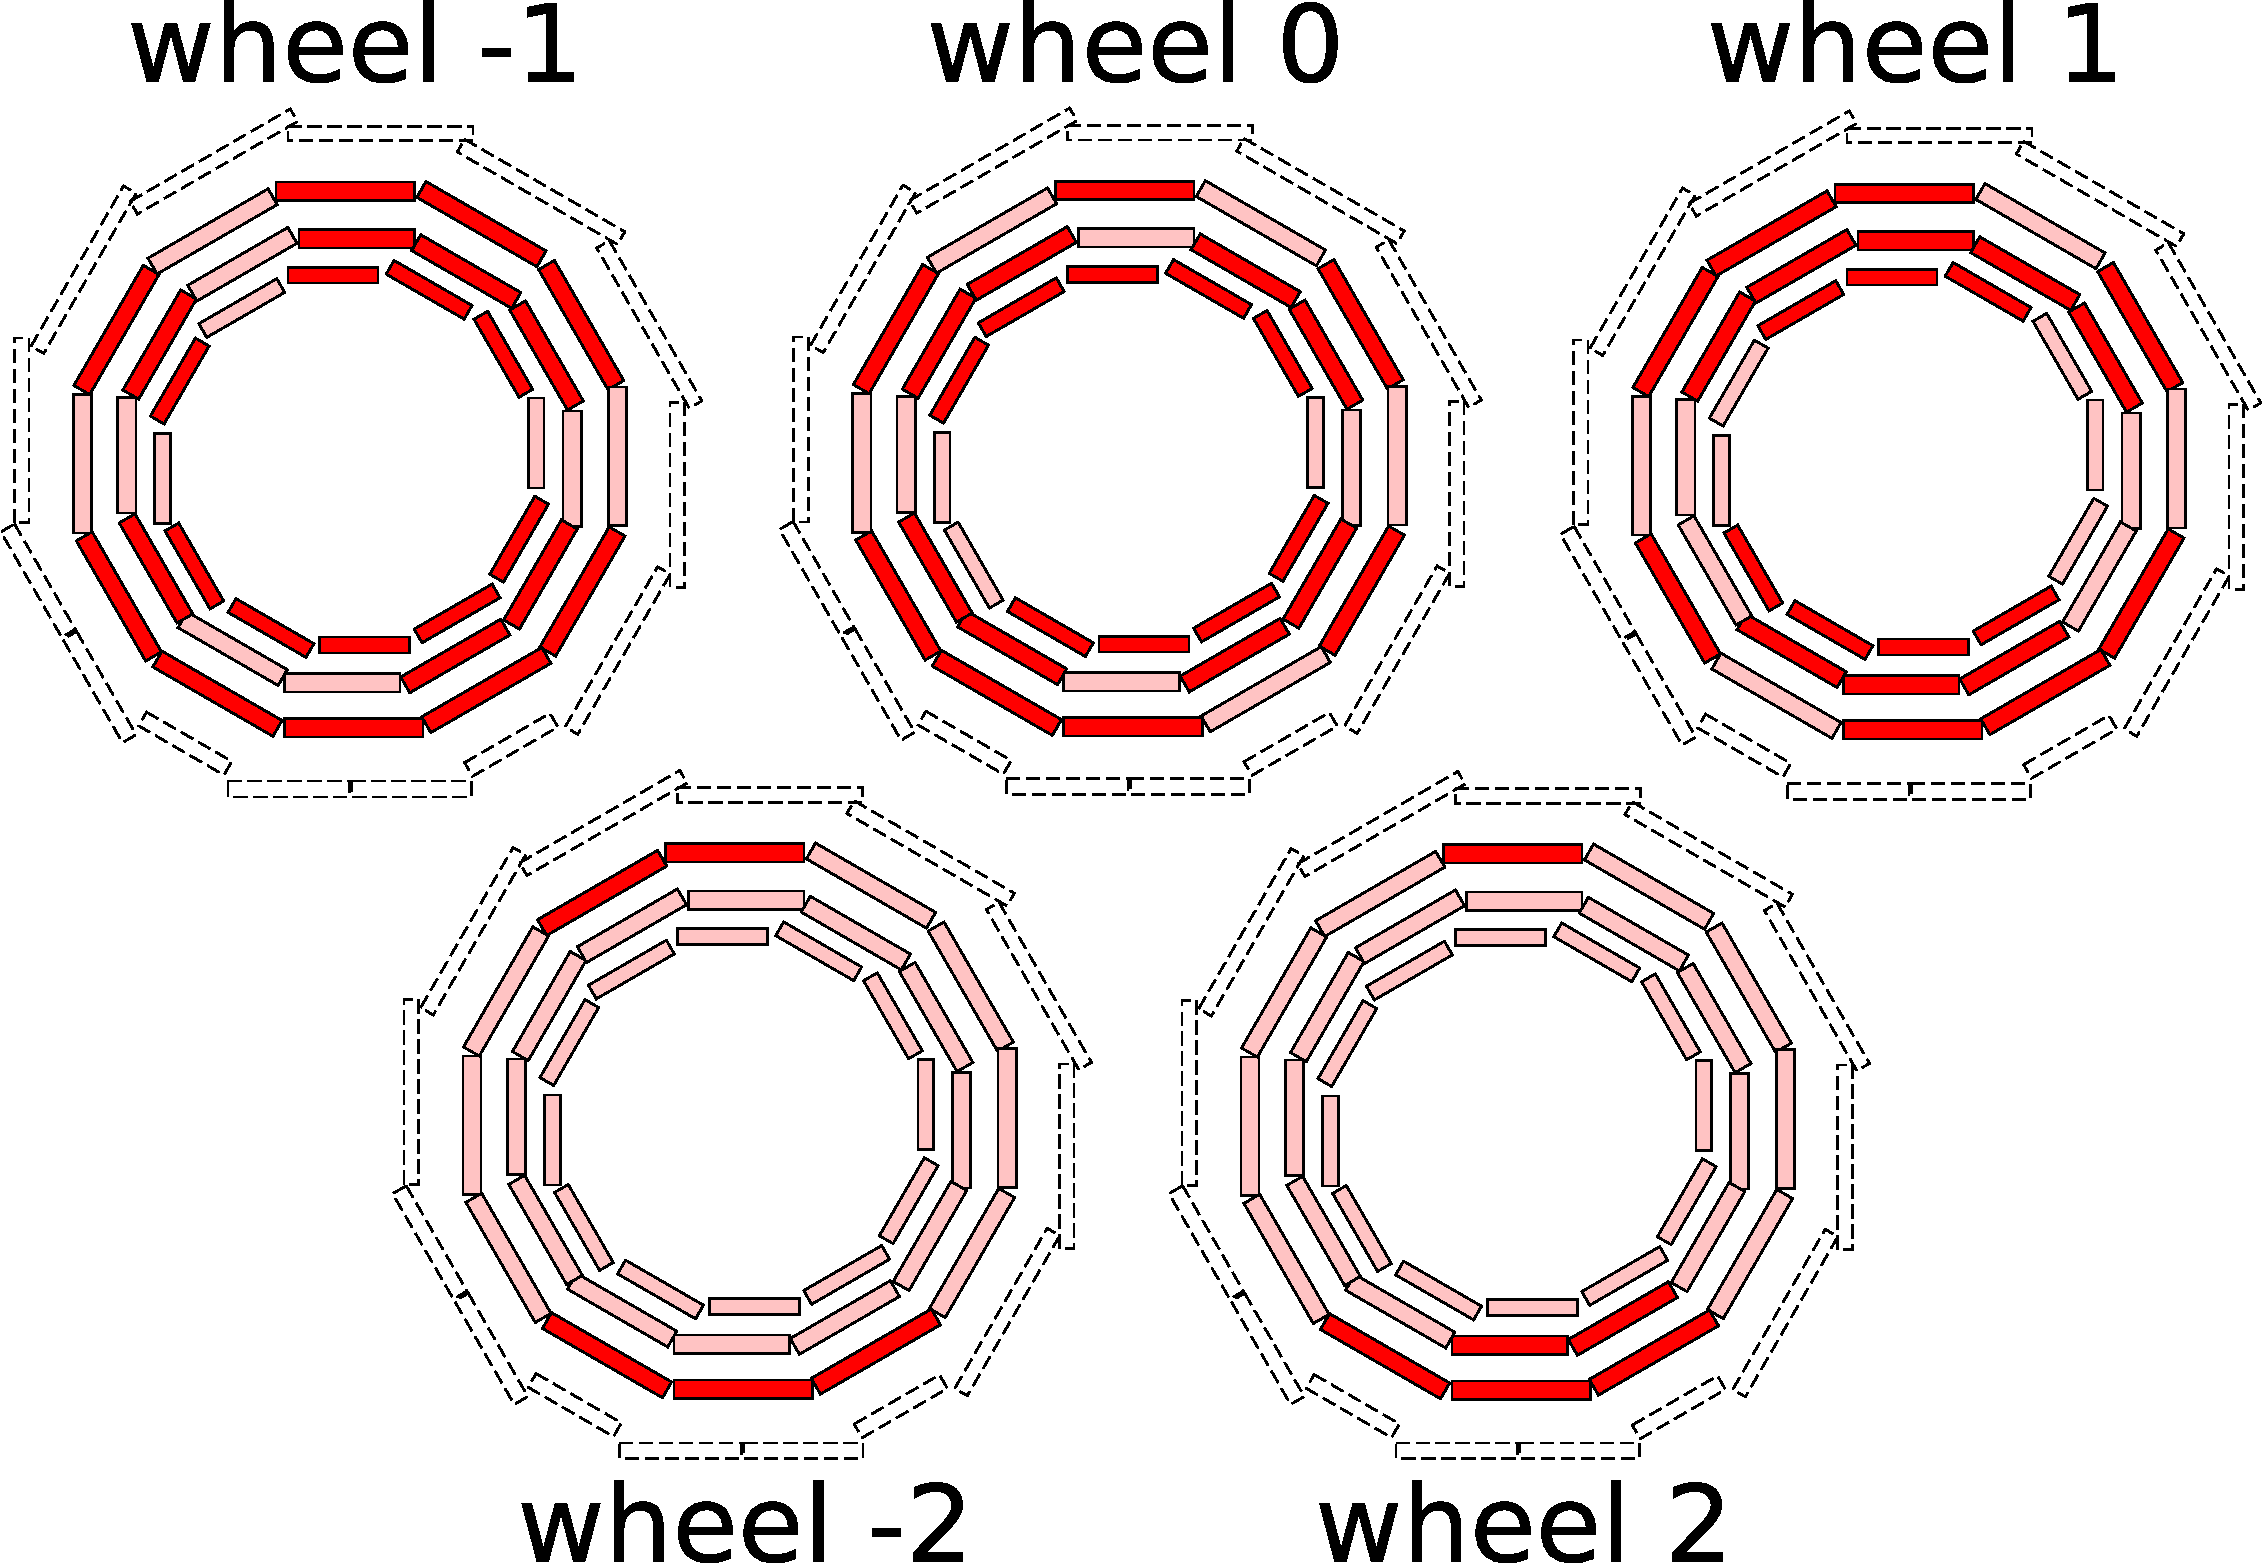
\includegraphics[width=0.45\linewidth]{aligned_z.pdf}
\end{tabular}

\vspace{-0.25 cm}
\begin{columns}
\column{0.35\linewidth}

\vspace{1 cm}
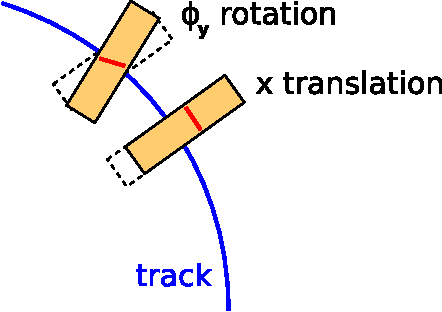
\includegraphics[width=\linewidth]{phiy_also_important.pdf}

\column{0.65\linewidth}
\begin{itemize}
\item Only chambers accessible to \mbox{globalMuons aligned\hspace{-1 cm}}
\begin{itemize}
\item \scriptsize many or most standAloneMuons cross both aligned and unaligned chambers
\item \scriptsize {\it shouldn't expect} improvement in standAloneMuons without controlling set of tracks and direction of fitting
\end{itemize}

\item Only three parameters: $x$, $\phi_z$, $y$
\begin{itemize}
\item \scriptsize $\phi_y$ angle is also important for measuring curvature (charge ratio analysis)
\end{itemize}
\end{itemize}
\end{columns}
\end{frame}

\begin{frame}
\frametitle{All 6 parameters from fits}

\begin{tabular}{c c}
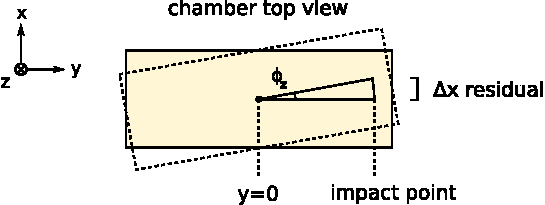
\includegraphics[width=0.5\linewidth]{phiz_diagram.pdf} & 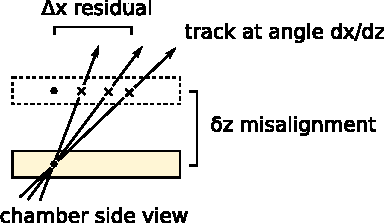
\includegraphics[width=0.4\linewidth]{zpos_diagram.pdf}
\end{tabular}

\vfill
\textcolor{darkblue}{\normalsize Four fits per chamber} ($\times$2 for two-bin $\vec{B}(\vec{x})$ and $dE/dx$ control)

\vspace{0.1 cm}
\renewcommand{\arraystretch}{1.35}
\begin{tabular}{p{0.5\linewidth} p{0.4\linewidth}}
Superlayer 1\&3 position residual & Superlayer 1\&3 angular residual \\\hline
\renewcommand{\arraystretch}{1.35}
\begin{tabular}{c c}
$x$ & central value \\
$\phi_z$ & slope w.r.t.\ $y$ position \\
$z$ & slope w.r.t.\ $\dfrac{dx}{dz}$ angle \\
sawtooth & slope w.r.t.\ angular residual \\
\end{tabular}
&
\begin{tabular}{c c}
$\phi_y$ & central value \\
\end{tabular} \\
& \\
Superlayer 2 position residual & Superlayer 2 angular residual \\\hline
\renewcommand{\arraystretch}{1.35}
\begin{tabular}{c c}
$y$ & central value \\
${\phi_z}$ & slope w.r.t.\ $x$ position \\
& {\it \tiny (cross-check superlayer 1\&3 $\phi_z$)} \\
\end{tabular}
&
\begin{tabular}{c c}
$\phi_x$ & central value \\
\end{tabular} \\
\end{tabular}
\end{frame}

\begin{frame}
\frametitle{Alignment software updates}

\begin{columns}
\column{0.4\linewidth}
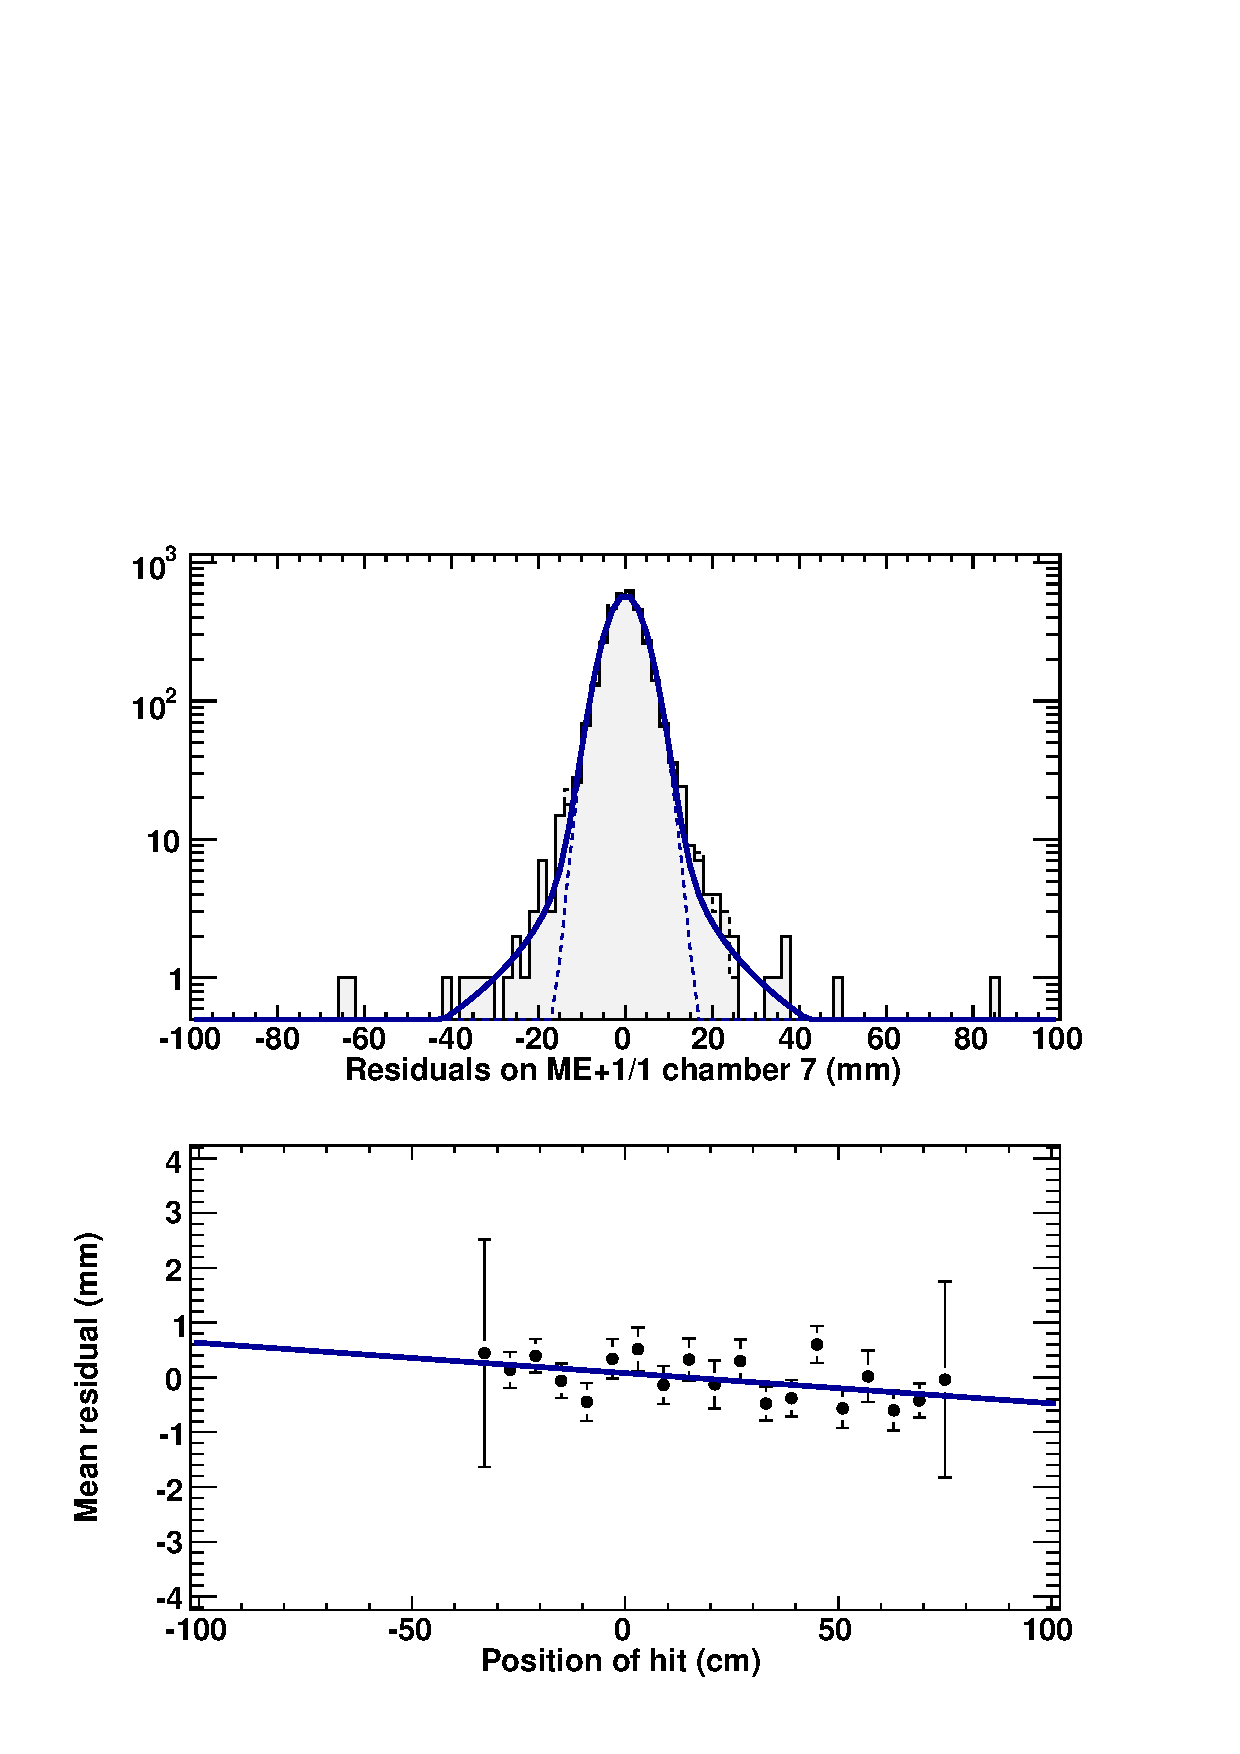
\includegraphics[width=\linewidth]{phizfit_demo_MEp11_7.pdf}

\vspace{0.25 cm}
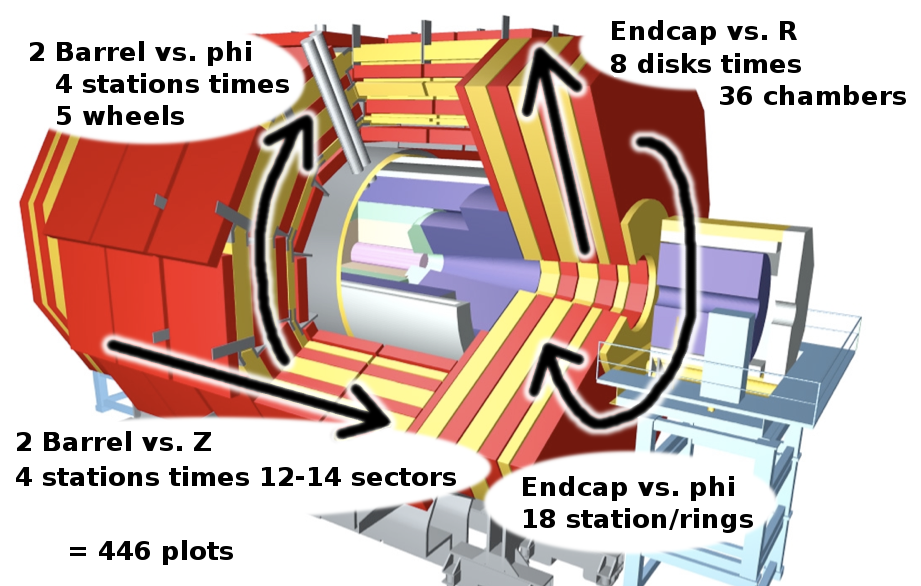
\includegraphics[width=\linewidth]{CMS_cutaway.png}

\column{0.6\linewidth}
\begin{itemize}\setlength{\itemsep}{-0.05 cm}
\item MuonAlignmentFromReference \mbox{now includes\hspace{-1 cm}}

\vspace{-0.2 cm}
\begin{itemize}
\item \scriptsize multiparameter fits (example on left)
\item \scriptsize endcap chambers
\end{itemize}

\item AlignmentMonitorMuonSystemMap

\vspace{-0.2 cm}
\begin{itemize}
\item \scriptsize DT residuals vs.\ $\phi$ and $z$
\item \scriptsize CSC residuals vs.\ $\phi$ and $R$ (below)
\end{itemize}

\item Tests in high-statistics MC reveal some biases

\vspace{-0.08 cm}
between propagator and GEANT

\vspace{-0.2 cm}
\begin{itemize}
\item \scriptsize several mm in local $z$ \mbox{(related to sawtooth?)\hspace{-1 cm}}
\item \scriptsize several hundred $\mu$m in $x$ in station~1 wheel~$\pm$2 (where $B_r$ is non-negligible)
\item \scriptsize related to $J/\psi$, $K_s$ mass biases?
\end{itemize}
\end{itemize}

\vspace{-0.2 cm}
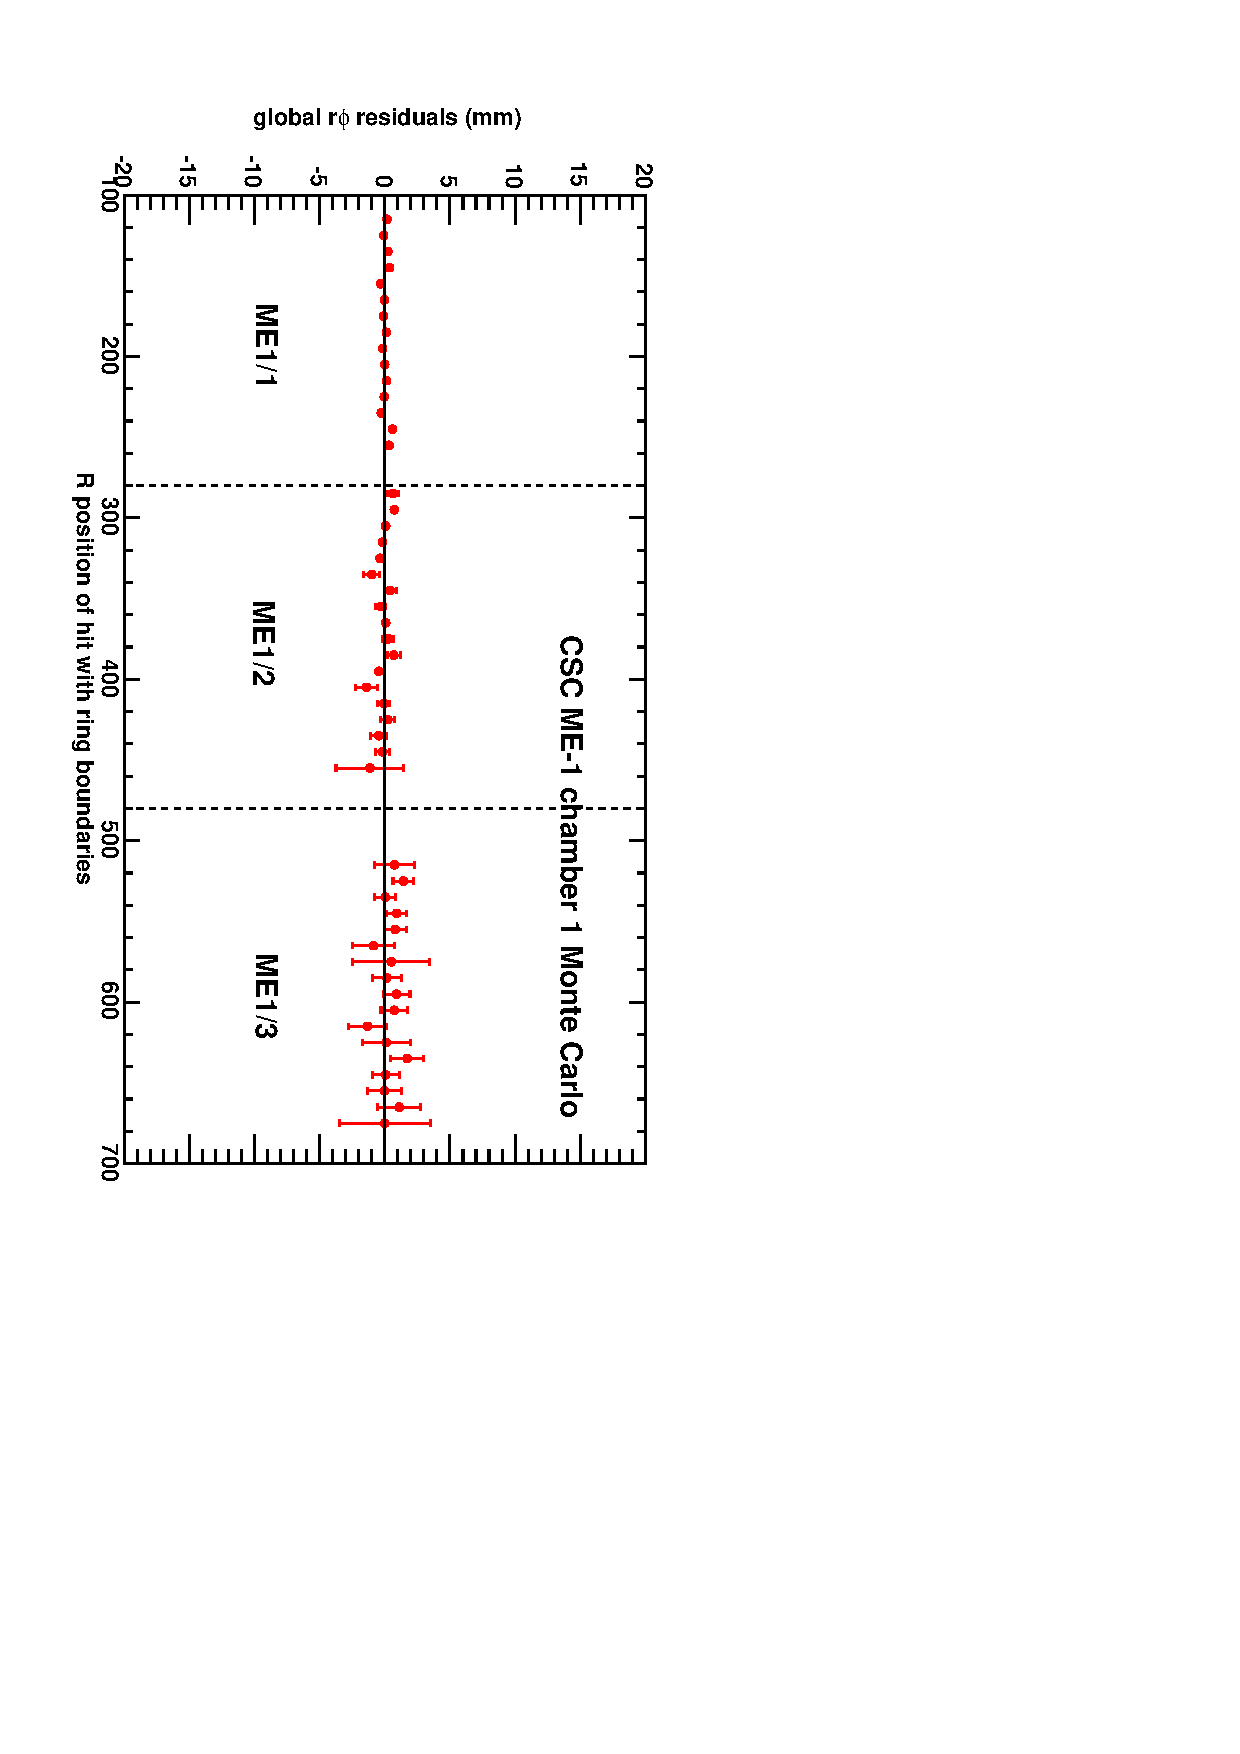
\includegraphics[height=\linewidth, angle=90]{CSCrphires_vsR_MEm1ch01_MC.pdf}

\end{columns}
\end{frame}

%% \begin{frame}
%% \frametitle{Importance of single scattering}

%% \begin{columns}
%% \column{0.55\linewidth}


%% \column{0.45\linewidth}
%% 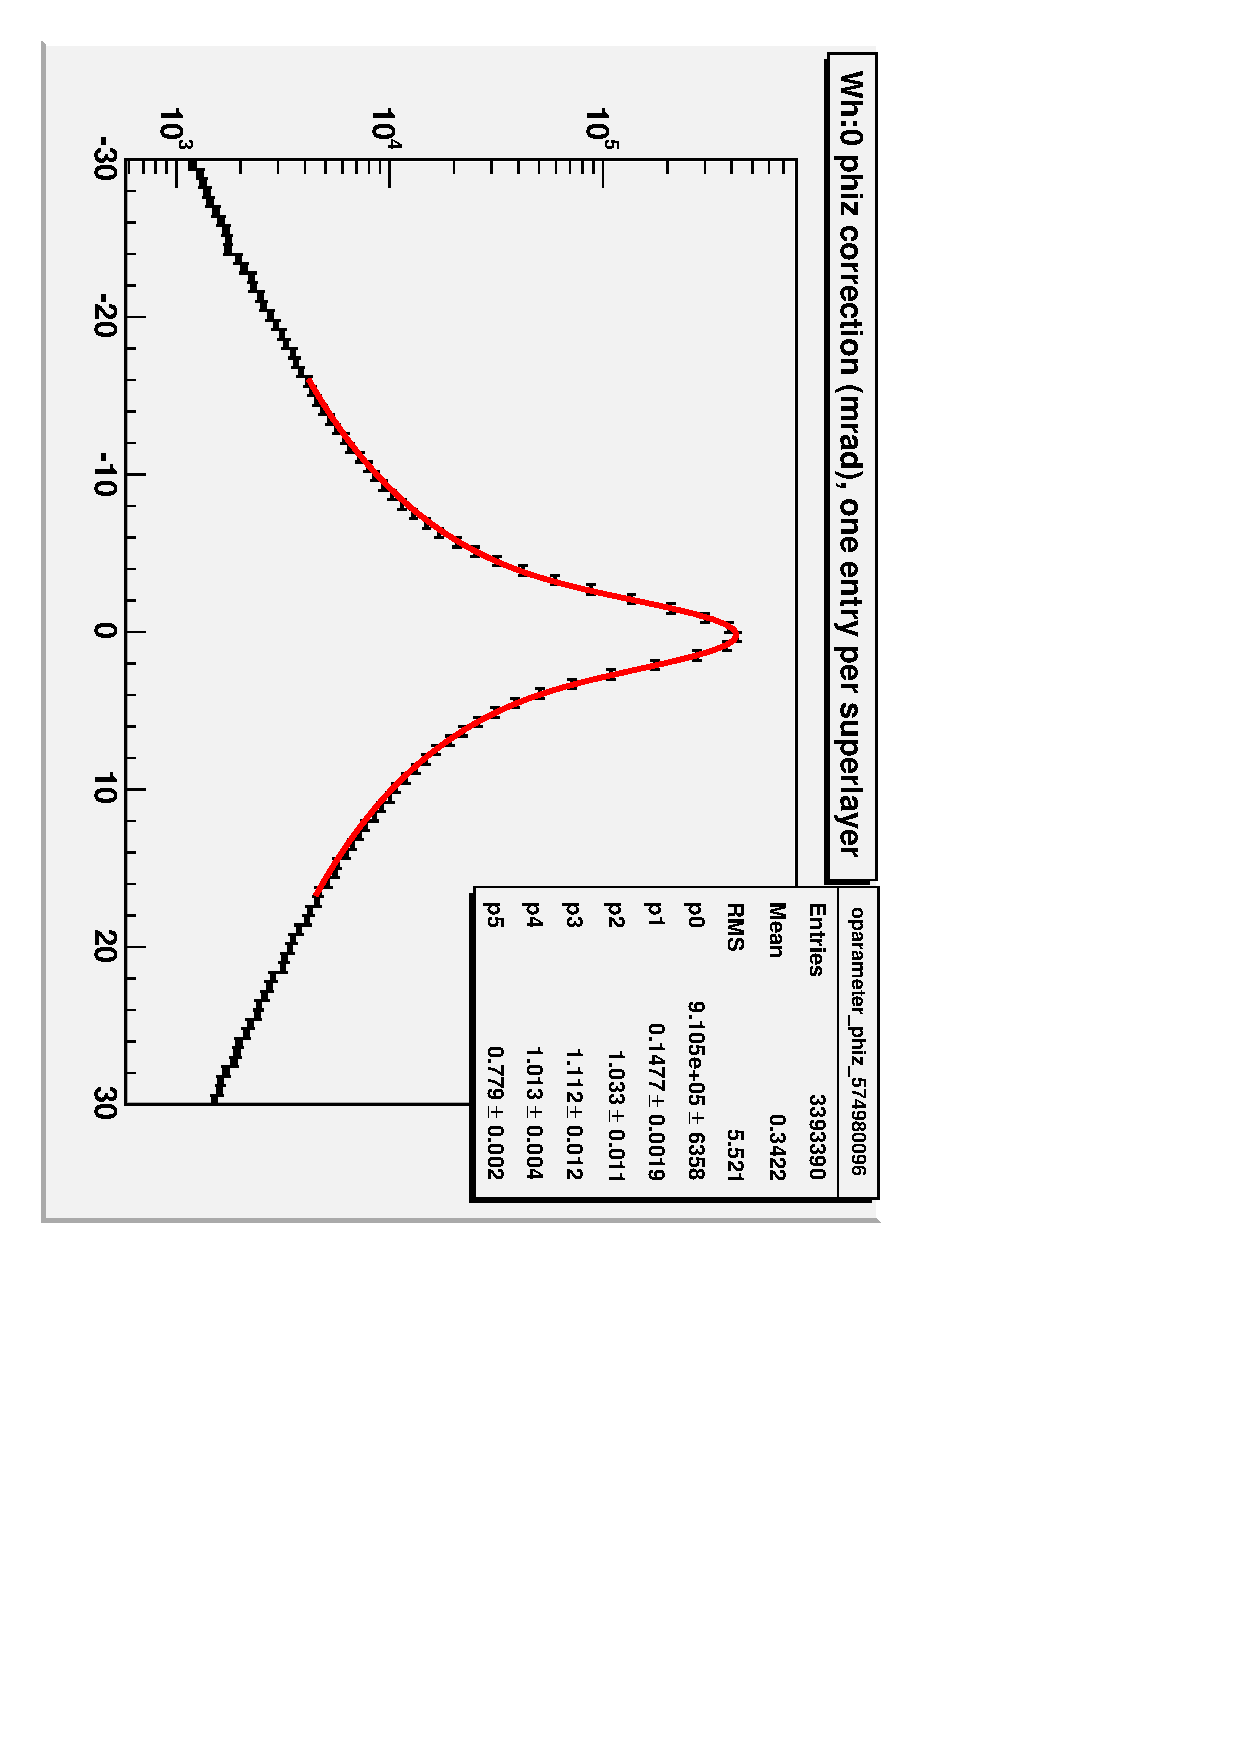
\includegraphics[height=\linewidth, angle=90]{fitfunction_superhighstats.pdf}
%% \end{columns}

%% \vfill
%% \begin{columns}
%% \column{0.4\linewidth}
%% \mbox{ } \hfill 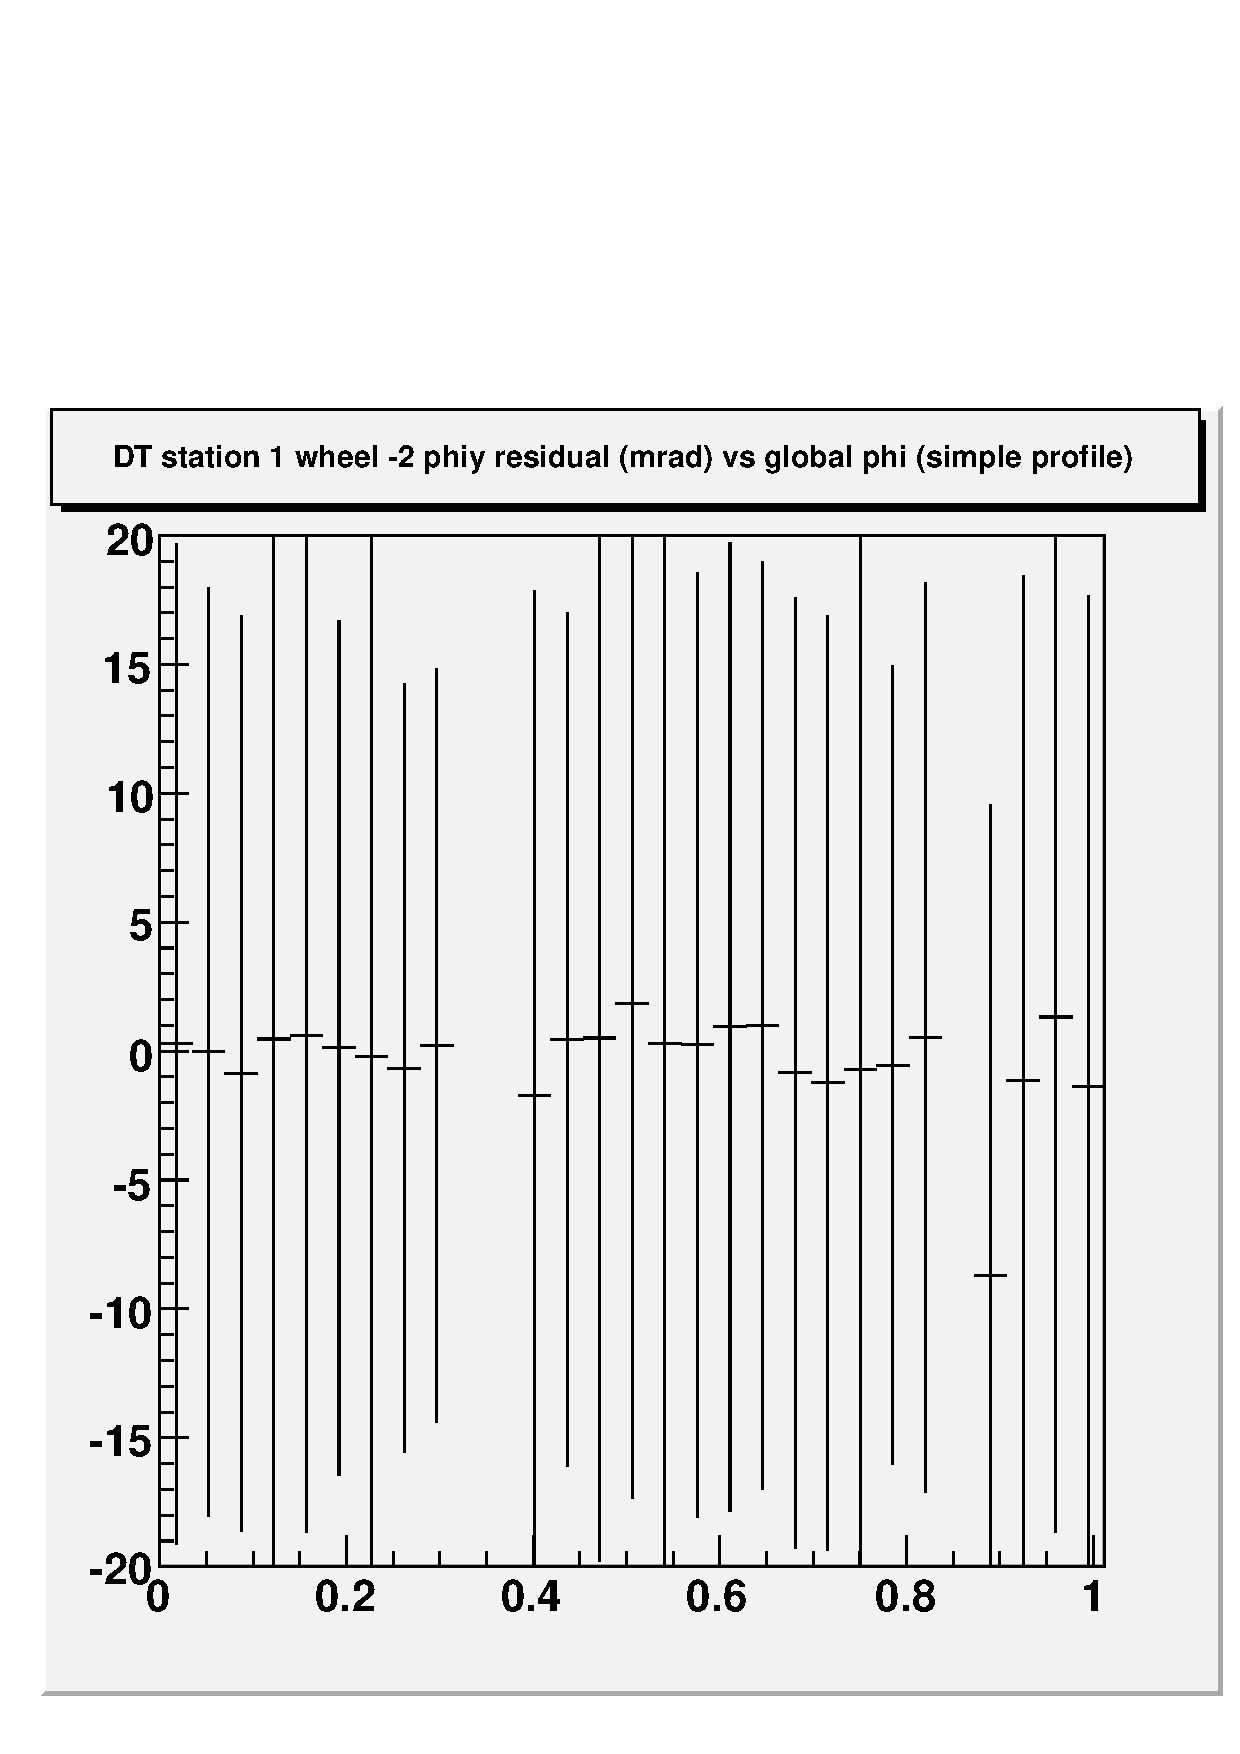
\includegraphics[width=0.75\linewidth]{tailfit_without.pdf}

%% \column{0.2\linewidth}
%% \begin{center}
%% Replace reasonably-truncated mean with tail-fit

%% \vspace{0.25 cm}
%% 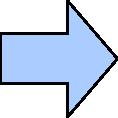
\includegraphics[width=0.5\linewidth]{arrow.pdf}
%% \end{center}

%% \column{0.4\linewidth}
%% 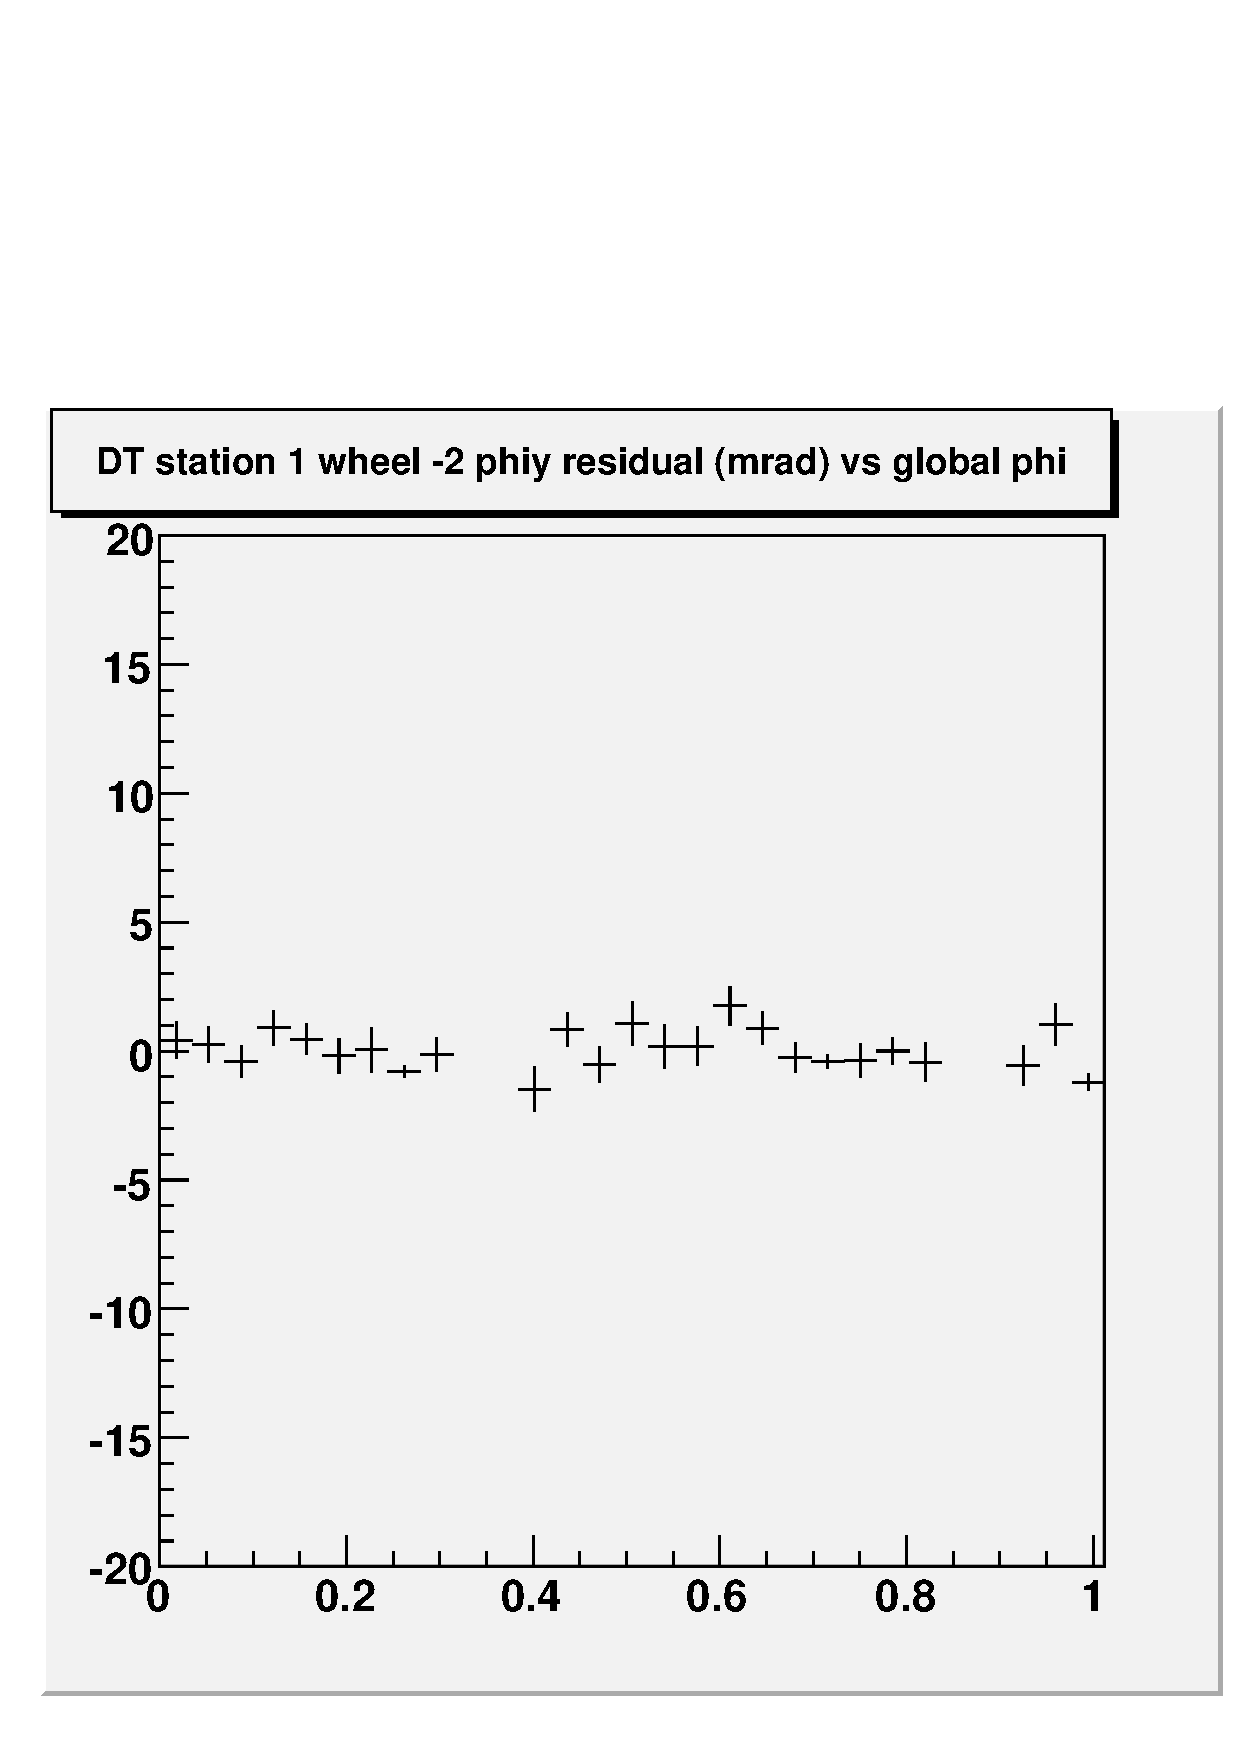
\includegraphics[width=0.75\linewidth]{tailfit_with.pdf} \hfill \mbox{ }
%% \end{columns}

%% \end{frame}

\begin{frame}
\frametitle{HIP and MillePede}
\begin{itemize}
\item The difference between Standard HIP and Standard MillePede
  algorithms is how they handle the feedback between track-fitting and
  alignment adjustments

\begin{center}
\renewcommand{\arraystretch}{1.25}
\begin{tabular}{c p{1 cm} c}
Standard HIP & & Standard MillePede \\\hline
alternate between track- & & solve combined problem \\
fitting and alignment & & as a large matrix
\end{tabular}
\end{center}

\item There's no such distinction for procedures which align to an external reference
\begin{itemize}
\item \scriptsize updating muon geometry doesn't affect tracker-only track fits
\item \scriptsize globalMuon-HIP and globalMuon-MillePede are the same algorithm
\end{itemize}

\item Two implementations of the same algorithm isn't an independent cross-check
\begin{itemize}
\item \scriptsize for the same reason that ``residuals $\to$ 0'' isn't an independent cross-check
\item \scriptsize only verifies that two people didn't make different mistakes
\item \scriptsize presentation of intermediate plots and constructive criticism can catch mistakes with only one implementation
\end{itemize}

\item Very local information (no propagation through iron) is \mbox{independent of globalMuons\hspace{-1 cm}}
\begin{itemize}
\item \scriptsize e.g.\ CSC Overlaps will severely check globalMuons approach in endcap
\item \scriptsize is something like a DT Overlaps possible?  (constrain neighboring {\it sectors} in the same station?)
\end{itemize}

%% \item Is similar complementarity possible in the barrel?
%% \begin{itemize}
%% \item \scriptsize MuonStandAloneAlgorithm aligns same 4 stations per track \mbox{as globalMuons\hspace{-1 cm}}
%% \item \scriptsize is it possible to link neighboring sectors in the same
%%   station with overlap segments? (analogy of
%%   CSCOverlapsAlignmentAlgorithm for DTs)
%% \end{itemize}

\end{itemize}
\label{numpages}
\end{frame}

%% \begin{frame}
%% \frametitle{Backup slide}

%% 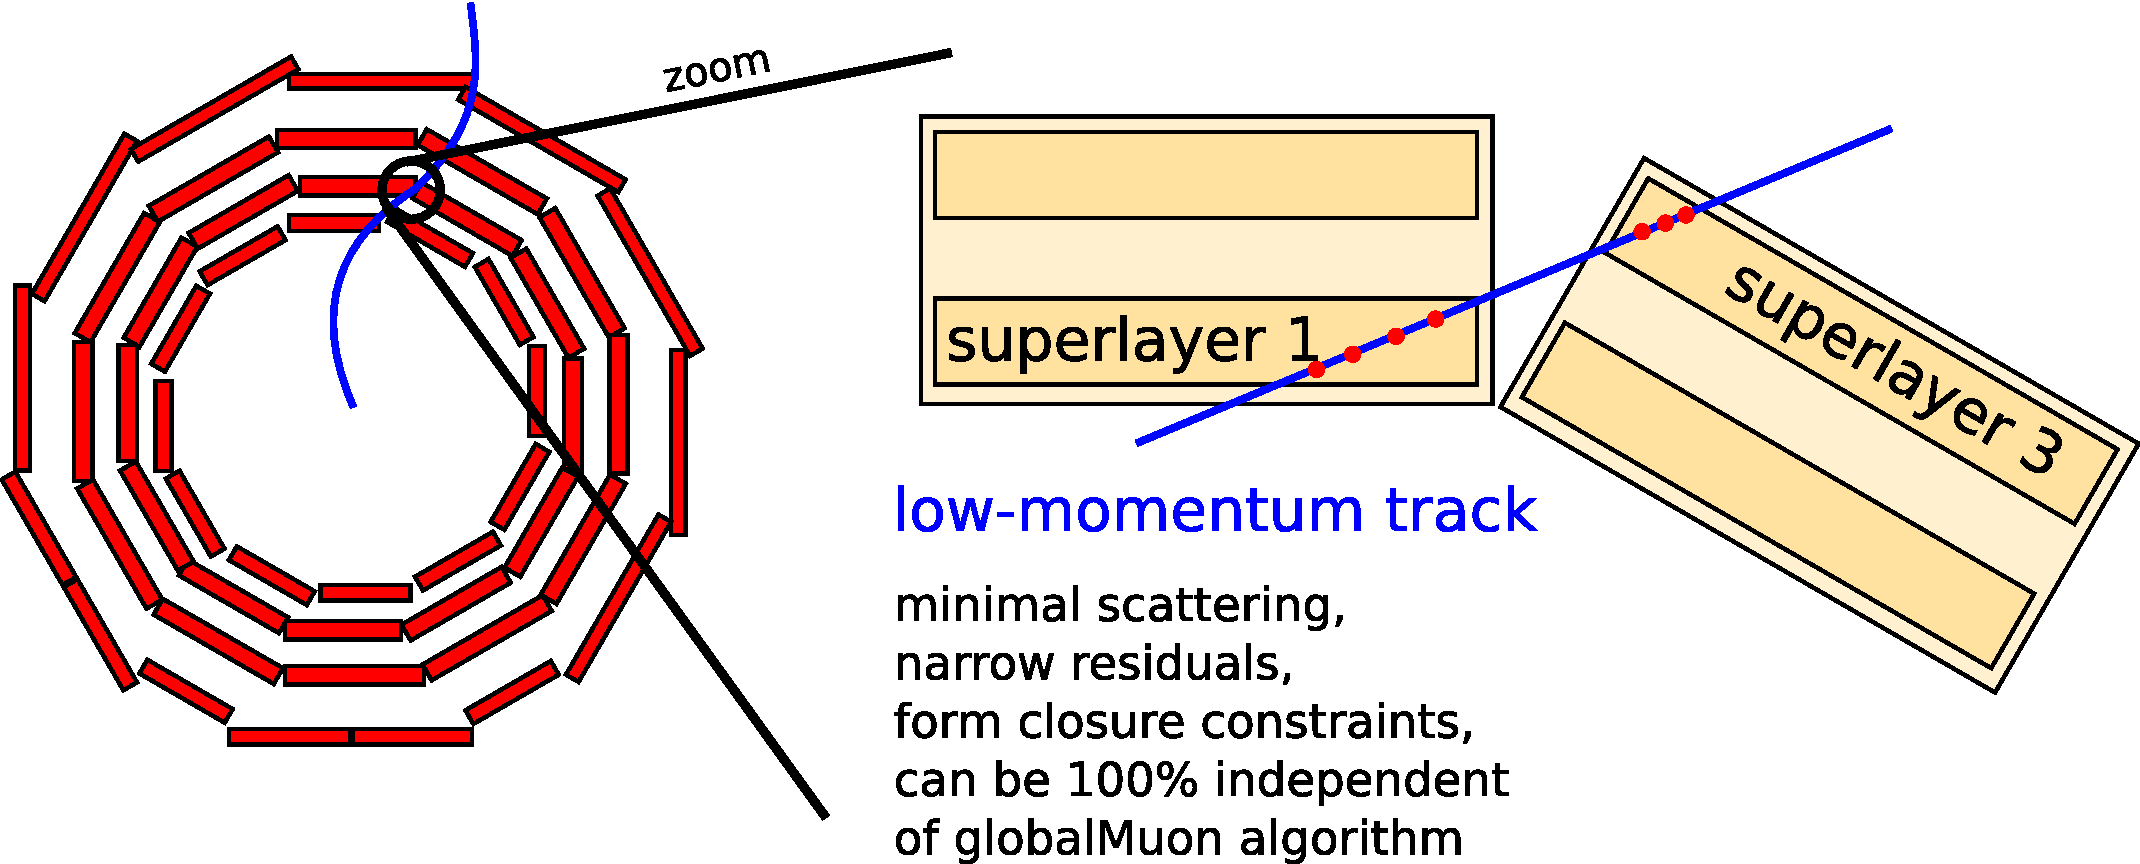
\includegraphics[width=\linewidth]{DToverlaps.pdf}
%% \end{frame}

%% \begin{frame}
%% \frametitle{Outline}
%% \begin{itemize}\setlength{\itemsep}{0.75 cm}
%% \item 
%% \end{itemize}
%% %% \hspace{-0.83 cm} \textcolor{darkblue}{\Large Outline2}
%% \end{frame}

%% \section*{First section}
%% \begin{frame}
%% \begin{center}
%% \Huge \textcolor{blue}{First section}
%% \end{center}
%% \end{frame}

%% \begin{frame}
%% \end{frame}

\end{document}
